%\documentclass{bioinfo}
%\copyrightyear{2019} \pubyear{2019}

%\access{Advance Access Publication Date: Day Month Year}
%\appnotes{Applications Note}

\documentclass[11pt]{article}

\usepackage{amsmath, amsfonts, amsthm}
\newtheorem{theorem}{Theorem}
\theoremstyle{definition}
\newtheorem{example}{Example}[section]

\usepackage[margin=1.25in]{geometry}
\usepackage{setspace}
\onehalfspacing
\usepackage{subfigure}
\usepackage{natbib}
\usepackage{graphicx}
\usepackage{authblk}

\setcounter{tocdepth}{2}

\begin{document}
%\firstpage{1}

%\subtitle{Genetic and population analysis}

% \title[Supplement to Unified GWAS power analysis]{Supplement to ``U-PASS: unified power analysis and forensics for qualitative traits in GWAS''}
\title{Supplement to ``U-PASS: unified power analysis and forensics for qualitative traits in gentic association studies''}
\author[1]{Zheng Gao\thanks{Corresponding author: gaozheng@umich.edu}}
\author[1]{Jonathan Terhorst}
\author[2]{Cristopher Van Hout}
\author[1]{Stilian Stoev}
\affil[1]{Department of Statistics, University of Michigan, Ann Arbor, MI 48109, USA}
\affil[2]{Regeneron Genetics Center, Tarrytown, NY 10591 USA.}
%\author[Gao \textit{et~al}.]{Zheng Gao\,$^{\text{\sfb 1,}*}$, Jonathan Terhorst\,$^{\text{\sfb 1}}$, Cris Van Hout\,$^{\text{\sfb 2}}$, and Stilian Stoev\,$^{\text{\sfb 1}}$}
%\address{$^{\text{\sf 1}}$Department of Statistics, University of Michigan, Ann Arbor, MI 48109, USA and \\
%$^{\text{\sf 2}}$Regeneron Genetics Center, Basking Ridge, NJ 07920, USA.}

%\corresp{$^\ast$To whom correspondence should be addressed.}

%\history{Received on XXXXX; revised on XXXXX; accepted on XXXXX}

%\editor{Associate Editor: XXXXXXX}

\maketitle

\vspace{-20pt}
\begin{abstract}
   We provide a brief overview of power analysis for genetic association studies in Section \ref{sec:power-analysis-overview}.
   The relationship between two approaches to specifying the alternative hypothesis in power calculations for association studies is clarified in Section \ref{sec:disease-models}.
   We develop a unified analysis of statistical power for common association tests in Section \ref{sec:asymptotic-equivalence}, and provide a simple rule for finite-sample correction of the asymptotic approximations in Section \ref{sec:finite-sample}.
   The performance of this correction is examined through numerical experiments in Section \ref{sec:numerical}.
   Proof of the main result is found in Section \ref{sec:proof}.
\end{abstract}

\tableofcontents

\section{Overview of power analysis in genetic association studies}
\label{sec:power-analysis-overview}
In power analysis of genetic association studies, disease models are used to specify the distribution of observations under the alternative hypothesis.
In this document, we discuss the challenges in disease model specifications, and discuss its relationship with an alternative approach that accomplishes the same goal through a set of "cannonical parameters".

We shall first briefly recall the main steps of a typical power analysis for genetic association studies.

\subsection{Disease model specifications}

A typical power analysis for genetic association studies begin by specifiying an alternative hypothesis through a disease model (dominant, recessive, multiplicative, additive, etc.), which assumes:

\begin{itemize}
    \item The genotype relative risks (GRR).
    \item Risk allele frequency in the general population ($p$).
    \item Disease prevalence in the general population (Prev).
\end{itemize}

The disease model and parameters determine the joint distribution of the genotypes and phenotyes {\it in the population}, shown in the following table.

\begin{center}
    \begin{tabular}{cccc}
    \hline
    & \multicolumn{3}{c}{Risk allele copies} \\
    \cline{2-4}
    Population Prob. & 0 copies & 1 copy & 2 copies \\
    \hline
    Cases & $\pi_{10}$ & $\pi_{11}$ & $\pi_{12}$ \\
    Controls & $\pi_{20}$ & $\pi_{21}$ & $\pi_{22}$ \\
    \hline
    \end{tabular}
\end{center}

In the disease models, the conditional probabilities of having the disease, given the risk allele copy numbers, satisfy the following relations,

\begin{equation} \label{eq:GRR}
    \frac{\pi_{10}}{\pi_{10} + \pi_{20}} : \frac{\pi_{11}}{\pi_{11} + \pi_{21}} : \frac{\pi_{12}}{\pi_{12} + \pi_{22}}
    = \begin{cases}
    1 : \text{GRR} : \text{GRR}^2, &\text{Multiplicative} \\
    1 : \text{GRR} : 2\times\text{GRR}-1, & \text{Additive} \\
    1 : \text{GRR} : \text{GRR}, & \text{Dominant} \\
    1 : 1 : \text{GRR}, & \text{Recessive}
\end{cases}
\end{equation}
where GRR is strictly greater than 1 under the alternative, and equal to 1 under the null hypothesis.

The disease prevalence determines the sum of the probabilities of cases in the population,
\begin{equation} \label{eq:prev}
    \pi_{10} + \pi_{11} + \pi_{12} = \text{Prev}.
\end{equation}

The risk allele frequency in the general population, $p$, assuming Hardy-Weinberg equilibrium, satisfies 
\begin{equation} \label{eq:RAF-pop}
    \pi_{10} + \pi_{20} = (1-p)^2, \quad \pi_{11} + \pi_{21} = 2p(1-p), \quad \pi_{12} + \pi_{22} = p^2.
\end{equation}

The population probabilities are determined by the disease model and its parameters (GRR, Prev, and $p$).
The six unknowns  $(\pi_{10},\ldots,\pi_{22})$ and are solved for using the six equations above: two from Relation \eqref{eq:GRR}, one from \eqref{eq:prev}, and three from \eqref{eq:RAF-pop}.


\subsection{Sampling adjustments}

Next, the probabilities of observing each genotype-phenotype combination are adjusted according the number of cases and controls recruited *in the studies*, where the sample sizes are specified with

\begin{enumerate}
    \item The number of cases ($n_1$) and controls ($n_2$), or equivalently, the fraction of cases ($\phi$) and total number of subjects ($n$).
\end{enumerate}


\begin{center}
    \begin{tabular}{cccc}
    \hline
    & \multicolumn{3}{c}{Risk allele copies} \\
    \cline{2-4}
    Prob. in study & 0 copies & 1 copy & 2 copies \\
    \hline
    Cases & $\pi_{10}\frac{\phi}{\text{Prev}}$ & $\pi_{11}\frac{\phi}{\text{Prev}}$ & $\pi_{12}\frac{\phi}{\text{Prev}}$ \\
    Controls & $\pi_{20}\frac{1-\phi}{1-\text{Prev}}$ & $\pi_{21}\frac{1-\phi}{1-\text{Prev}}$ & $\pi_{22}\frac{1-\phi}{1-\text{Prev}}$ \\
    \hline
    \end{tabular}
\end{center}

As an example, if $\phi > \text{Prev}$, the probabilities are adjusted to account for over-sampling of cases.

The relative frequencies of allele type-phenotype combinations {\it in the study} are then calculated as follows.

\begin{center}
    \begin{tabular}{ccc}
    \hline
    & \multicolumn{2}{c}{Allele variant} \\
    \cline{2-3}
    Prob. in study & Risk allele & Non-risk allele \\
    \hline
    Cases & $\phi\left(\frac{\pi_{12}}{\text{Prev}}+\frac{\pi_{11}}{2\times\text{Prev}}\right)$ & $\phi\left(\frac{\pi_{11}}{2\times\text{Prev}}+\frac{\pi_{10}}{\text{Prev}}\right)$ \\
    Controls & $(1-\phi)\left(\frac{\pi_{22}}{1-\text{Prev}}+\frac{\pi_{21}}{2(1-\text{Prev})}\right)$ & $(1-\phi)\left(\frac{\pi_{21}}{2(1-\text{Prev})}+\frac{\pi_{20}}{1-\text{Prev}}\right)$ \\
    \hline
    \end{tabular}
\end{center}

To simplify notation, we denote the relative frequencies of allele type-phenotype combinations with $\mu = (\mu_{11}, \mu_{12}, \mu_{21}, \mu_{22})$.


\begin{center}
    \begin{tabular}{cccc}
    \hline
    & \multicolumn{2}{c}{Allele variant} & \\
    \cline{2-3}
    Prob. in study & Risk allele & Non-risk allele & Total by phenotype \\
    \hline
    Cases & $\mu_{11}$ & $\mu_{12}$ & $\phi = \mu_{11} + \mu_{12}$ \\
    Controls & $\mu_{21}$ & $\mu_{22}$ & $1-\phi = \mu_{21} + \mu_{22}$ \\
    \hline
    \end{tabular}
\end{center}

\subsection{Power calculations of association tests}

Finally, the power of an statistical test is calculated as the probability of (a correct) rejection, assuming that the data (i.e., tabulated counts of the allele type-phenotype combinations) follow a multinomial distribution with probability matrix $\mu$ and sample size $2n$, since each individual has a pair of alleles.

% \footnote{Caveat: The final step in the power calculations does not apply to association tests performed directly on the 2-by-3 contingency tables of phenotype-genotype combinations (e.g., the Cochran-Armitage test).Therefore, the GAS calculator should not be used if these tests are to be applied.}.

Some common association tests include the likelihood ratio test, Pearson's chi-square test, tests of zero slope coefficient in logistic regressions, as well as t-tests for equal proportions.
In principal, power analysis has to be tailored to the association test used.
Fortunately, many of these tests are asymptotically equivalent in terms of power, and results of the power analysis applies to all equivalent tests; see Section \ref{sec:asymptotic-equivalence}.

These steps form the basis of the calculations implemented in the most existing tools, including the GAS calculator \citep{Johnson17}.
Although not explicitly stated, the GAS calculator assumes the test of association to be the Welch t-test.



\section{Two approaches to specifying the alternative hypothesis}
\label{sec:disease-models}
In the power calculations outlined above, the disease models are used to describe the distribution of the data under the alternative hypothesis.
Specifically, they are used to specify the conditional distributions of the allele variants, given the phenotypes.
The probability of observing a risk allele in the control group,
\begin{equation}
    f := \mathbb{P}[\,\text{risk allele}\,|\,\text{control group}\,] 
    = \frac{\mu_{21}}{1-\phi} 
    = \frac{\pi_{22} + \pi_{21}/2}{\pi_{22} + \pi_{21} + \pi_{20}},
\end{equation}
is fully determined by the disease model.
Similarly, the odds ratio between the two allele variants, 
\begin{equation}
    R:=\frac{\mu_{11}\mu_{22}}{\mu_{12}\mu_{21}} 
    = \frac{(\pi_{12} + \pi_{11}/2)(\pi_{20} + \pi_{21}/2)}{(\pi_{10} + \pi_{11}/2)(\pi_{22} + \pi_{21}/2)},
\end{equation}
is also determined by the disease model and its parameters.

In turn, the parameters $(f, R)$, together with the sample sizes $(\phi, n)$, fully describe the distribution of our data under the alternative hypothesis (by determining the probability vector $\mu$ and the sample size $n$).
Power of association tests, therefore, depends on (and only on) the set of ``canonical parameters'':

\begin{itemize}
    \item Risk allele frequency among the controls (f).
    \item Odds ratio (R) of having the defined trait between the two allele variants.
    \item One of the two equivalent ways of parametrizing the sample sizes.
\end{itemize}

We illustrates the common process of power analysis implemented in existing power calculators in Figure \ref{fig:flowchart}.

\begin{figure*}[!tpb]
    \centering
    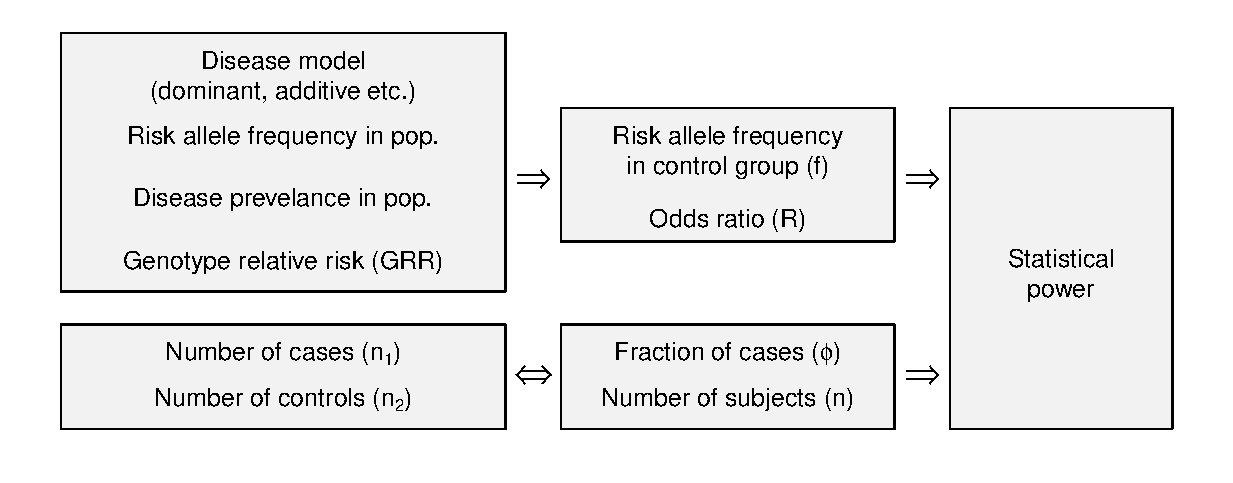
\includegraphics[width=\textwidth]{flowchart.eps}
    \caption{The process of a typical power analysis for genetic association tests.
    The quantities depend on, and can be calculated from the values of their parents in the directed graph. 
    Power can be calculated as long as one set of parameters in each branch is known.
    While there is a one-to-one correspondence between the sample size specifications $(n_1, n_2)$ and $(\phi, n)$, the mapping from disease model specifications to $(f, R)$ is many-to-one. 
    %That is, one cannot recover the disease model specifications from the allelic tables, or equivalently, reported risk allele frequencies and odds ratios.
    }
    \label{fig:flowchart}
\end{figure*}

Our discussion above shows that in power calculations, {\it we can either describe the alternative hypothesis with a disease model, or through the canonical parameters ($f, R$). Both approaches are sufficient for the purpose of power analysis.}

We remind readers that the risk allele frequency in the control group ($f$) is not equivalent to the risk allele frequency in the general population ($p$); odds ratio ($R$) is not equivalent to genotype relative risk (GRR).


\subsection{Conversion between the two specifications}

Notice that, as illustrated in  Figure \ref{fig:flowchart}, the power calculations are mediated through the canonical parameters, which are invariant to different model specifications.
That is, different disease model specifications may lead to the {\it same} set of canonical parameters ($f, R$), and consequently the) {\it same} distributions of the allele variant counts.
From a statistical perspective, the disease models that map to the same set of canonical parameters are equivalent in terms of power.

For example, the following set of disease models and parameters imply the same set of canonical parameters $(f = 0.290, R = 1.575)$, and therefore enjoy the same power at the same sample sizes ($n_1 = n_2 = 1000$).
\begin{center}
    \begin{tabular}{cc|cc}
    \hline
    Disease Model & $(\text{Prev}, p, \text{GRR})$ & $(f, R)$ & Power \\
    \hline 
    Multiplicative & $(0.1, 0.3, 1.500)$ & $(0.290, 1.575)$ & 0.990 \\
    Additive & $(0.1, 0.3, 1.588)$ & $(0.290, 1.575)$ & 0.990 \\
    Dominant & $(0.1, 0.3, 1.909)$ & $(0.290, 1.575)$ & 0.990 \\
    Recessive & $(0.1, 0.3, 2.666)$ & $(0.290, 1.575)$ & 0.990 \\
    \hline
    \end{tabular}
\end{center}

Conversely, different disease models with the same parameters, map to drastically different canonical parameters.
For example, the default disease model parameters in the GAS calculator,
\begin{align}
    \text{Disease prevalence in the population}: & \quad \text{Prev} = 0.1 \\
    \text{Risk allele frequency in the population}: & \quad p = 0.5\\
    \text{Genotype relative risk}: & \quad \text{GRR} = 1.5.
\end{align}
map to very different canonical parameters under different disease model assumptions (assuming the same sample sizes of $n_1 = n_2 = 1000$), which leads to drastically different statistical power.
\begin{center}
    \begin{tabular}{cc|cc}
    \hline
    Disease Model & $(\text{Prev}, p, \text{GRR})$ & $(f, R)$ & Power \\
    \hline 
    Multiplicative & $(0.1, 0.5, 1.5)$ & $(0.489, 1.568)$ & 0.995 \\
    Additive & $(0.1, 0.5, 1.5)$ & $(0.491, 1.453)$ & 0.920 \\
    Dominant & $(0.1, 0.5, 1.5)$ & $(0.495, 1.224)$ & 0.282 \\
    Recessive & $(0.1, 0.5, 1.5)$ & $(0.494, 1.281)$ & 0.098 \\
    \hline
    \end{tabular}
\end{center}

In the application, we provide users with a ``Disease model converter'' that implements this many-to-one conversion from the disease model specifications to the canonical parameters.


\subsection{Comparisons of the two approaches}
\label{subsec:comparing-two-approaches}

While the disease models may carry additional insights into the biological process, the canonical parameters also have their unique advantages.
We offer an incomplete list of comparisons of the two approaches, and discuss their usage in practice.

\subsubsection{Interpretability and communicability}

In general, geneticists and biostatisticians seem to agree that disease models are more interpretable.
The concept of genotype relative risks, in particular, seems easier to reason about than odds ratios in the canonical parameters definition.
Disease models also seem to be the de facto mode of model specification when performing power analysis for study planning and grant applications.

The ``nonparametric'' approach to model specification through the canonical parameters is somewhat lesser known to the statistical genetics community.
The canonical parameters are typically estimated and reported as outcomes of the research, but not used as inputs to the power analysis for planning purposes.

\subsubsection{Availability of parameter estimates}

The canonical parameters $f$ and $R$ can be estimated from data collected in the study.
They are also reported and curated in GWAS catalogs such as the NHGRI-EBI Catalog \citep{MacArthur16}.

On the other hand, accurate information regarding the disease model parameters can be more difficult to obtain, partly because some parameters in the disease models cannot be estimated from the association studies alone.

In particular, disease prevalence in population (Prev), as well as RAF in population ($p$), must be obtained from other studies or surveys targeting the general population; the association studies, unless matching the proportion of cases in the population vs in the study ($\phi=\text{Prev}$), cannot produce estimates without using external information.
Genetic association studies rarely explicitly estimate the disease model and its parameters.
In fact, we are not aware of a GWAS catalog that reports and curates the disease models and their estimated parameters.

This paucity of information on disease model parameters is not an issue if we are planning to study a trait for which we have little prior knowledge.
In this case, the purpose of power analysis is to determine the range of models and parameters that lead to discovery of associations, given the study designs.

In contrast, in confirmatory / follow-up studies and systematic reviews, our main interest is in the statistical validity of the reported findings.
Power analysis then serves to find efficient designs, and to validate the claims made.
Knowledge obtained in prior studies (in the form of parameter estimates) are indeed necessary.

\subsubsection{Robustness against model misspecification}

Disease models are useful in as much as they help us understand the biology behind the data we observe.
Unfortunately, like all models, they can be misspecified. 
For example, the following genotype relative risks,
\begin{equation*}
    \frac{\pi_{10}}{\pi_{10} + \pi_{20}} : \frac{\pi_{11}}{\pi_{11} + \pi_{21}} : \frac{\pi_{12}}{\pi_{12} + \pi_{22}}
    = 1 : 3 : 4,
\end{equation*}
does not follow any of the common disease models.
In this case, different studies may come up with different disease models (say, Dominant and Additive), and of course, different parameter estimates.

Suppose a researcher wishes to perform a meta analysis or confirmatory experiment of the existing results, where the literature reports inconsistent estimates of disease models and parameters,
he would a have a difficult time pooling the information from these different sources. 
And even when they are pooled, the resulting model usually does not fall in one of the familiar categories --- there is no existing tool with which to perform power analysis.
The researcher will likely have to forgo the information from one model, and use estimates from only the other.

On the other hand, the canonical parameters are invariant to the disease model choices, and accommodate models falling outside the usual categories. 
They can also be easily combined to produce pooled estimates.
This universality allows us to perform power analysis in a unified fashion, regardless of the disease models assumed.
This also paves the way for the ``OR-RAF diagram'', as well as systematic reviews of statistical validity of existing studies.

\subsubsection{Robustness against human errors}

The disparity in availability of parameter estimates we mentioned earlier can lead to unintended consequences, one of which is potentially incorrect usage of power calculators.

This issue, although minor, affects correctness of the results from power analysis.

Recall that the specification of a disease model requires as input the risk allele frequency (RAF) in the general population ($p$).
The RAF reported in the NHGRI-EBI Catalog \citep{MacArthur16}, in contrast, refers to RAF in the control group ($f$).
With RAF in population often unavailable, it is tempting to substitute the RAF in control group into the calculations.
While the two quantities may be close when diseases prevalence and penetrance are low, their difference becomes non-negligible if either of the two conditions are violated, leading to grossly distorted results.

Performing power analysis with the canonical parameters is not guaranteed to prevent this human error, as mistake in the other direction could also happen.
But perhaps it is more robust to such mistakes, since what is readily available matches with what is required as input.

\subsubsection{Compatibility of parameters}

We make another minor comment regarding correct usage of disease models.

We caution users that not all values of the disease model parameter combinations are valid.
For example, in a multiplicative model, the parameters 
\begin{equation*}
    p = 0.1, \quad \text{Prev} = 0.5, \quad \text{GRR} = 1.5,
\end{equation*}
would result in the conditional probability of having two risk allele copies greater than 1.
(In this case, the GAS calculator \citep{Johnson17} would produce the error message: ``I don't like the genetic model you requested!'', without explicitly pointing to the compatibility issue.)

Although an experienced geneticist would immediately notice the impossibility of the disease model parameter combinations, these contradictions may not be obvious to the untrained eye.
The end user of the software -- experienced or not -- is ultimately responsible for inputting valid values when specifying a disease model.

On the other hand, any combination of 
\begin{equation*}
    f\in(0,1), \quad \text{and} \quad R\in(0,+\infty)
\end{equation*}
is valid. 
Parameter compatibility is not an problem for the set of canonical parameters.

\subsection{Recommendations on model specification in power analysis}

Since both the disease models and the canonical parameters are sufficient for the purpose of power analysis, a natural question then arises: why (and when) should one take the canonical parameters approach, given that the more familiar disease models would also suffice?

We believe that either approach may be preferred, depending on the use cases.
Recall that power analysis is useful in at least three scenarios:
\begin{enumerate}
    \item {\it In planning for an exploratory study, where little is known about the associations.}
    
    In this case, the top branch in Figure \ref{fig:flowchart} is unknown to the researcher.
    The goal is to find out the range of disease models and parameters that are discoverable given the study designs.
    Power analysis is also to some extent exploratory in nature.
    
    \item {\it In planning for a confirmatory study, where something is known about the associations and one wishes to validate the findings with an efficient design.}
    
    In this case, the top branch in Figure \ref{fig:flowchart} is known, and the variables in the bottom branch is what we are solving for.
    The goal of power analysis is to provide a set of efficient study designs with sufficient power.
    
    \item {\it In reviewing the reported findings and verify the statistical validity of the claims made.}
    
    In the third case, one looks to find out whether the claims of statistical significance are congruent with the evidence from data.
    A claim supported by very weak or contradictory evidence should invite further investigations.
    In this case, both branches in Figure \ref{fig:flowchart} have to be available.
\end{enumerate}

In view of the discussions above and in Section \ref{subsec:comparing-two-approaches}, we propose the following general guideline for power analysis in genetic association studies.

\begin{itemize}
    \item When designing an association study where little to no prior information is available: 
    \begin{itemize}
        \item Either approach is valid.
        \item Disease models are easier to interpret and communicate.
    \end{itemize}
    \item When designing a follow-up / confirmatory study, or conducting a systematic review:
    \begin{itemize}
        \item Choose the approach for which the parameter estimates are available, or of better quality.
        \item Typically the canonical parameters are better estimated, reported, and curated.
    \end{itemize}
\end{itemize}
% The simple answer is the following: the canonical parameter approach is better suited to planning confirmatory studies and performing systematic reviews, which to the best of our knowledge, could not be readily done prior to our tool. 
There are, of course, exceptions to these rules.
The minor comments we made about the two approaches should not be taken as criticisms, but rather as reminders of the potential pitfalls in power analysis.
In either approach, care needs to be exercised in order to produce valid results.



\section{Use case illustrations}
\label{sec:user-guide}

We detail each of the three functionalities of the application, and illustrate with examples.

\subsection{Reviewing reported findings in the GWAS catalog}

The ``OR-RAF power diagram'' tab of the application provides a tool for reviewing reported associations from existing studies.
The application calculates statistical power based the core parameters common to models of qualitative traits:

\begin{itemize}
    \item Sample sizes, i.e., the number of cases and controls i.e., $(n_1, n_2)$ or $(\phi, n)$.
    \item The canonical parameters $(f, R)$.
\end{itemize}

Users need only prescribe the sample sizes, by one of two ways provided in the first box, i.e., total sample size + fraction of cases, or number of cases + number of controls.

Statistical power of familiar association tests, including the likelihood ratio test, chi-square test, Welch's t-test, and LR test for logistic regressions, have the same asymptotic power curves
(see the Section \ref{sec:asymptotic-equivalence} for details).
This common power limit is calculated as a function of RAF and OR, and visualized as a heatmap in the OR-RAF diagram. 

\subsubsection{Adaptive and interactive display for exploring GWAS catalogs}

We provide options for users to load and overlay findings reported in the NHGRI-EBI GWAS Catalog \citep{MacArthur16}, or upload data from other sources compliant with the Catalog's data format.

The initial sample sizes are dynamically adjusted, and automatically determined from texts of the article reporting the user selected loci.
Since the sampling structures are many and varied across different studies, and no uniform reporting format is enforced in the catalog, the initial sample sizes are best estimates from the extracted texts.

Information of the selected loci and the study is also dynamically displayed below the diagram.

\subsubsection{An example: forensics of existing studies}

The unified power analysis allows us to examine results from different studies employing different models and applicable tests, in the same diagram, with the same power limits.
It allows for a systematic review of reported findings for their statistical validity.

In particular, a reported association predicted to have low power given the study's sample size -- lying in the dark regions of the OR-RAF diagram -- while not impossible, invites further scrutiny. 

It should be noted that a reported association predicted to have high power is not automatically accurate, as survival bias induced by multiple testing may inflate the reported OR and RAF estimates.

Studies where reported associations show misalignment with the predicted powered curves may be further investigated for potential problems in the data curation process.
The following figure shows one such study, where gross misalignment was identified.

\begin{figure*}[!tpb]
    \centering
    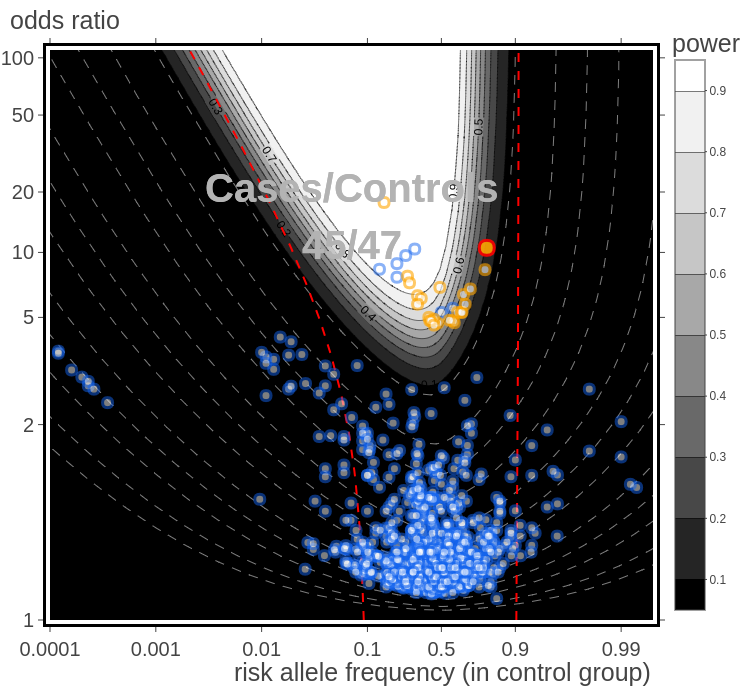
\includegraphics[width=0.6\textwidth]{forensics.png}
    \caption{
    One study where gross misalignment was identified \citep{Dominguez-Cruz18}. 
    We reached out to the authors of the study, who confirmed that this is the result of a problem in the data curation process of the GWAS Catalog (Dominguez-Cruz, personal communication). 
    In particular, the RAF reported in the Catalog were based on all subjects in the study, as opposed to only the control group, while the Catalog requires that RAF be reported in the control group only. 
    As a consequence, the RAFs are systematically overestimated, shifting the reported findings to the right in the diagram.
    }
    \label{fig:forensics}
\end{figure*}

In general, we expect this aspect of our software to be useful for discovering problems with data entry and catalog curation process, as well as for assessing the reproducibility and robustness of reported findings.

\subsection{Designing association studies}

The ``Design my studies'' tab of the application provides a tool for finding optimal designs of association studies.
The tool requires inputs in a four-step process.
\begin{enumerate}
    \item Model specification.
    \item Sample size constraints specification.
    \item False discovery Criteria specification.
    \item Target power specification.
\end{enumerate}
Each of the steps can be specified in a number of alternative ways.

\subsubsection{Model specification}

We provide two three ways to describe the model for biological process of the disease or trait of interest.

As outlined in Section \ref{sec:disease-models}, the distribution of observations can be specified through the canonical parameters, risk allele frequency in the control group ($f$) and odds ratio ($R$).
Estimates for these quantities in previous studies of the same trait can be found in GWAS catalogs such as the NHGRI-EBI Catalog.
See Section \ref{sec:disease-models} for their definitions.

Alternatively, users may opt to specify through the disease models, of which we implement the four most popular ones: additive, multiplicative, dominant, and recessive.
See Section \ref{sec:power-analysis-overview} for the definitions of the quantities involved in the disease models.
We remind users the difference between the risk allele frequency in the control group ($f$) versus risk allele frequency in the general population ($p$); only the latter is used in the disease model specifications.

Advanced users may choose to use a more succinct ``signal size per sample'' option, which directly parametrizes the signal sizes ($\lambda/n$).
Details can be found in Section \ref{sec:proof}.

\subsubsection{Sample size specifications}

The second step requires users input the sample size constraints of the study.
The three available options are ``Budget / total number of subjects'', ``Number of cases'', and ``Fraction of cases''.
In the subsequent calculations, the selected and specified quantities are treated as fixed.
With only one unknown parameter left in the flow of power calculations (recall the flowchart in Fig. \ref{fig:flowchart}), we calculate power as a function of the  remaining specified parameter.
In particular,

\begin{itemize}
    \item If the constraint is total budget, power is shown as a function of the fraction of cases.
    \item If the constraint is number of cases, power is shown as a function of the number of controls.
    \item If the constraint is fraction of cases, power is shown as a function of the total number of subjects.
\end{itemize}

\subsubsection{Type I and Type II errors specifications}

The final two steps require as input the desired level of false discovery and false non-discovery control.
Both specification can be done through the marginal levels, i.e., Type I error and Type II error, or alternatively, through the multiple testing-adjusted levels, i.e., family-wise error rate (FWER) and family-wise non-discovery rate (FWNR).

\subsubsection{An example: designing prospective studies}

A researcher wishes to find out how many controls are needed in order to detect an association between a risk variant described by a multiplicative model with parameters:
$$
\text{RGG} = 1.2, \quad p = 0.3, \quad \text{Prev} = 0.1.
$$
The study has recruited 1000 subjects in the case group, and is aiming for power of 80\% with FWER controlled at 5\% level adjusted for the multiplicity of $10^6$ tests.

In the application, we input the disease model parameters in the first step.
In the second step, we select the sample size constraint as ``number of cases'' and set to 1000.
The third step, we selected FWER as the criteria, and set the appropriate levels and multiplicity; a p-value cut off ($0.05/10^6=5\times10^{-8}$) is automatically calculated and displayed.
The final step, we choose ``Type II error / (1-power)'' as the target and select $1-80\%=20\%$.

The result of the calculation shows that the targeted power cannot be achieved at the current number of cases, no matter how many controls are recruited.
Therefore, the researcher should consider recruiting more subjects in the case group in order to in crease power.
For example, if there are instead 4000 subjects in the case group, then we would need only roughly 4929 controls in order to achieve the desired level of power.


\subsection{Converting disease models into canonical parametrization}

The ``Disease model converter'' tab of the application provides a tool for converting disease models into their implied canonical parameters.

The converter implements the mapping from disease models to the canonical parameters as detailed in Section \ref{sec:disease-models} and  illustrated in Figure \ref{fig:flowchart}.
The tool also allows users to copy the model parameters into the ``Design my study'' tab for power calculations.
Several numerical examples, discussed in Section  \ref{sec:disease-models}, are provided in the tool. 



\section{Unified asymptotic analysis of power}
\label{sec:asymptotic-equivalence}
In genetic association studies, researchers have the freedom to choose their favorite statistical procedure to perform hypothesis tests with the data collected.
In this section, we answer the natural question that arises: does the choice of statistical test influence the power of scientific discovery?

It turns out, perhaps unsurprisingly, that most common association tests have asymptotically equivalent power. 
We shall quantify this shared power limit, and provide practical formulas for power calculations.

\subsection{A model-invariant parametrization}

In association studies for qualitative traits, counts of subjects in each phenotype-genetic variant combination are tabulated in the form of a contingency table.
For a 2-allele-variant-by-2-phenotype definition, we have the following table of counts.

\begin{center}
    \begin{tabular}{cccc}
    \hline
    & \multicolumn{2}{c}{Genotype} & \\
    \cline{2-3}
    \# Observations & Variant 1 & Variant 2 & Total by phenotype \\
    \hline
    Cases & $O_{11}$ & $O_{12}$ & $n_1$ \\
    Controls & $O_{21}$ & $O_{22}$ & $n_2$ \\
    \hline
    \end{tabular}
\end{center}

Statistics are then calculated based on the counts, to test for associations between the genotypes and phenotypes, at levels adjusted for multiplicity.
Performance of a test is measured in terms of power, i.e., probability of correct rejection under an alternative hypothesis.

As we have seen in Section \ref{sec:disease-models}, power analysis typically starts by assuming an alternative distribution, typically (though not necessarily) described by a disease model.
Power of a test is approximated either based on large sample asymptotics, or by simulating the empirical distribution of the statistic under the alternative.

Recall the 2-by-2 multinomial distributions with probability matrix $\mu = (\mu_{ij})_{2\times2}$,
\begin{center}
    \begin{tabular}{cccc}
    \hline
    & \multicolumn{2}{c}{Allele type} \\
    \cline{2-3}
    Prob. in study & Risk allele & Non-risk allele & Total by phenotype \\
    \hline
    Cases & $\mu_{11}$ & $\mu_{12}$ & $\phi = \mu_{11} + \mu_{12}$ \\
    Controls & $\mu_{21}$ & $\mu_{22}$ & $1-\phi = \mu_{21} + \mu_{22}$ \\
    \hline
    \end{tabular}
\end{center}

We may assume -- by relabelling, and hence without loss of generality -- that allele Variant 1 is positively associated with the Cases, and referred to as the risk allele/variant. 

The multinomial probability matrix $\mu$ can be fully parametrized by the parameter triple:

\begin{itemize}
    \item Fraction of Cases $\phi$, i.e., marginal distribution of phenotypes.
    \item Conditional distribution of risk variant among Controls, i.e., risk allele frequency (RAF) in the Control group 
    \begin{equation} \label{eq:risk-allele-frequency}
    f := \mu_{21}/(1-\phi).
    \end{equation}
    \item Odds ratio (OR) of the allele Variant 1 to Variant 2
    \begin{equation} \label{eq:odds-ratio}
    \text{R} := \frac{\mu_{11}}{\mu_{21}}\Big/\frac{\mu_{12}}{\mu_{22}}
    = \frac{\mu_{11}\mu_{22}}{\mu_{12}\mu_{21}}.
    \end{equation}
\end{itemize}

An alternative hypothesis, e.g., a disease model, determines the canonical parameters $(f, R)$ implicitly,
%The fraction of Cases $\phi$ is part of the study design.
and therefore fully determines statistical power for a specific test at given sample sizes.
Alternatively, power can also be calculated by directly prescribing the canonical parameters and the sample sizes.

It is worth pointing out that while disease models play no role beyond specifying the alternative, they do sometimes inform our choice of a test statistic, hence influencing statistical power in higher order contingency tables.
These tests include, e.g., the Cochran-Armitage test, and variations thereof;
see \cite{Gonzalez08, Li08} for further examples where tests are tailored to disease models. 

We make the important distinction between RAF \emph{in the Control group} ($f$), versus RAF \emph{in the study} ($\mu_{11}+\mu_{21}$), and RAF \emph{in the general population} ($p$).
In the following sections, unless otherwise stated, RAF will refer to the risk allele frequency in the Control group, consistent with the reporting standards of the NHGRI-EBI Catalog \citep{MacArthur16}.

\subsection{Conditional vs unconditional tests}

Readers familiar with the underlying assumptions of association tests in contingency tables may have noticed that we have described a multinomial distribution of the cell counts.
That is, we have only conditioned on the total number of observations in the study.
This is indeed the assumption behind tests such as (the original, unconditional version of) the likelihood ratio test, and the Person chi-square test.

It is not, however, the assumption behind some other tests.
For example, analysis of t-tests typically assumes the observed number in each arm of the study are given.
That is, we would condition on the phenotype marginals when comparing the proportions of genetic variants among the Cases and Controls.
It is perhaps an assumption most close to reality, where the number of samples collected in each arm of the study are pre-determined.
In this case, we have two binomial observations, Binom$(n_1, p_1)$ and Binom$(n_2, p_2)$, instead of a multinomial observation.
\begin{center}
    \begin{tabular}{cccc}
    \hline
    & \multicolumn{2}{c}{Allele type} \\
    \cline{2-3}
    Cond. Prob. & Variant 1 & Variant 2 & Counts by phenotype \\
    \hline
    Cases & $p_{1}$ & $1-p_{1}$ & $n_1$ \\
    Controls & $p_{2}$ & $1-p_{2}$ & $n_2$ \\
    \hline
    \end{tabular}
\end{center}
RAF and OR can be similarly defined,
\begin{itemize}
    \item Marginal distribution of Cases, fixed at $\phi := n_1/(n_1+n_2)$,
    \item Risk allele frequency (RAF) in the Control group is the synonymous with the conditional distribution of risk variant among Controls, $$f := p_2,$$
    \item Odds ratio (OR)
    $$\text{R} := \frac{p_{1}\phi}{p_{2}(1-\phi)}\Big/\frac{(1-p_{1})\phi}{(1-p_{2})(1-\phi)}
    = \frac{p_{1}(1-p_{2})}{(1-p_{1})p_{2}}.
    $$
\end{itemize}
Alternative hypotheses may be formed as in the multinomial case with parameters $\phi$, $f$ and $R$, along with the total samples size.

Finally, we mention the assumptions behind the Fisher's exact test.
The Fisher exact test conditions on the number of observations of both the phenotype variants and genetic variants, leading to a hypergeometric distribution of the first cell count $O_{11}$ given the marginals $n_1$, $n_2$, and $O_{11}+O_{21}$, under the null hypothesis.
We found no easy parametrizations of alternative hypotheses under this framework.
Indeed, existing power calculations for Fisher's exact test resort to simulations under the two-binomial assumptions \citep{Smyth17}.

We refer interested readers to the recent work by \citet{Ripamonti17} and \citet{Choi17} which elucidate the controversies regarding the choices of conditioning when performing statistical inferences on 2-by-2 contingency tables.
We do not attempt to resolve the controversies in this work.
Our goal is to state clearly the assumptions behind the tests, and show the asymptotic equivalence in terms of power, under their respective assumptions.

\subsection{A test-independent power analysis}
\label{subsec:power-calculation}

We now present the main result allowing a unified power analysis, applicable for a wide range of common association tests in 2-by-2 tables.
% This is formalized in Theorem \ref{thm:1} below, where we show a number of tests enjoy the same power asymptotically.
% This unifies, and simplifies power calculations.

If we consider a fixed parameter values of $(f, R)$ under the alternative, no matter how close to the null, the probability of rejection of the null hypothesis by any reasonable test should approach one as sample size increases ($n\to\infty$).
On the other hand, the probability of rejection is less than one in finite samples, making this type of asymptotics useless for approximation.

Therefore, in order to find finer approximations of power, we study alternatives close to the null.
In particular, we take a sequence of alternatives approaching a limit point in the null space, in the hope that limiting rejection probability is between 0 and 1.
It turns out -- see, e.g., \citet{Ferguson17} Chapter 10, and \citet{Lehmann04} Chapter 5 -- that the appropriate rate at which the alternatives should shrink towards the limit point is $1/\sqrt{n}$. % and the appropriate limit point is the maximum likelihood estimate (MLE) of the probabilities under the null hypothesis (which happens to coincide with the minimum chi-square estimates).

Under the multinomial assumption, let $\mu^{(0)}$ be the probability matrix of the (independent) 2-by-2 multinomial distribution, with marginals $(\theta, 1-\theta)$ for the genetic variants, and marginals $(\phi, 1-\phi)$ for the phenotypes.
We require that $\theta\in(0,1)$ and $\phi\in(0,1)$ be bounded away from 0 and 1.
Let $\mu = \mu^{(n)}$ be the sequence of alternatives such that 
\begin{equation} \label{eq:alternative-multinomial}
    \sqrt{n}(\mu^{(n)} - \mu^{(0)}) \rightarrow \delta \begin{pmatrix} 1 & -1 \\ -1 & 1 \end{pmatrix},
\end{equation}
where $\delta$ is a positive constant.

Equivalently, under the two-binomial assumption, let $p_1^{(0)} = p_2^{(0)} = \theta$ be the null hypothesis, with fixed marginals $(\phi, 1-\phi)$ for the phenotypes.
Let $(p_1, p_2) = p^{(n)}$ be the sequence of alternatives such that 
\begin{equation} \label{eq:alternative-two-bionomial}
    \sqrt{n}\phi (p_1-\theta) \rightarrow \delta
    \quad \text{and} \quad 
    \sqrt{n}(1-\phi) (p_2-\theta) \rightarrow -\delta,
\end{equation}
where $\delta$ is a positive constant.
It is easy to see that with the same $\delta$ the two sequences of alternatives have the same RAF and OR, and therefore have the same expected number of observations in each cell.

\begin{theorem} \label{thm:1}
In 2-by-2 contingency tables, under the assumption that the counts in the contingency table follow the multinomial distributions.
%\vspace{-5pt}
\begin{itemize}
    \item The likelihood ratio test for independence,
    \item the likelihood ratio test for zero slope in logistic regressions,
    \item Person's chi-squared test for Independence,
\end{itemize}
%\vspace{-5pt}
and under the assumption that counts in the contingency table follow the two binomial distributions, 
%\vspace{-5pt}
\begin{itemize}
    \item the two-sided Welch's t-test for equal proportions 
\end{itemize} 
%\vspace{-5pt}
have the same asymptotic power curves.
Specifically, for the sequence of alternatives defined in \eqref{eq:alternative-multinomial} and \eqref{eq:alternative-two-bionomial}, all of the listed tests, at level $\alpha$, have statistical powers converging to 
\begin{equation} \label{eq:power-approx}
    \mathbb P[\chi^2(\lambda) \ge q_{\alpha}],
\end{equation}
where $q_{\alpha}$ is the upper $\alpha$ quantile of the central chi-square distribution, and $\chi^2(\lambda)$ is a non-central chi-square distribution with non-centrality parameter
\begin{equation} \label{eq:non-centrality}
    \lambda = \delta^2/{(\theta(1-\theta)\phi(1-\phi))}.
\end{equation}
\end{theorem}

The proof of Theorem \ref{thm:1} is detailed in Section \ref{sec:proof} below.

Theorem \ref{thm:1} is the central result that paves the way for a unified power analysis.
It allows us to chart findings from different studies employing the applicable tests in the same diagram, with the same power limits.
In particular, for large samples, tests for zero slopes in logistic regressions should report approximately the same set of loci as Welch's t-tests for equal proportions on the same dataset, after the same family-wise error rate adjustments.
The estimated odds ratios (in the case of logistic regression, estimate slopes exponentiated) and RAF's, when charted on the OR-RAF diagram, should also follow the same power limits.

To use this result for power calculations, we start with an alternative hypothesis, defined by the canonical parameters $(f, R)$, and sample sizes $(\phi, n)$.
\begin{center}
    \begin{tabular}{ccc}
    \hline
    & \multicolumn{2}{c}{Allele type} \\
    \cline{2-3}
    Probabilities & Variant 1 & Variant 2 \\
    \hline
    Cases & ${fR\phi}/{(fR+1-f)}$ & ${(1-f)\phi}/{(fR+1-f)}$ \\
    Controls & $f(1-\phi)$ & $(1-f)(1-\phi)$ \\
    \hline
    \end{tabular}
\end{center}
Elementary algebra yields $\theta = {fR\phi}/{(fR+1-f)} + f(1-\phi)$, and $\delta = \sqrt{n}(\theta - f)(1-\phi)$.
If tests are based on allele type counts, accounting for the fact that each genetic location has a pair of alleles, the effective sample sizes should be doubled, and the appropriate non-centrality parameter becomes  $\delta = \sqrt{2n}(\theta - f)(1-\phi)$.
Power may then be approximated using the formula in \eqref{eq:power-approx}.
% We conjecture that all aforementioned tests are asymptotically equivalent, in both the multinomial and two-binomial framework.




\section{Finite-sample corrections}
\label{sec:finite-sample}

The result of our power calculations above are only accurate to the extend that the asymptotic approximations are applicable.
In practice, of course, we have only finite samples, and the asymptotic approximations no longer hold when cell counts are low.
While existing tools have completely ignored this issue, we offer here a simple correction in finite samples by resorting to exact tests.

Specifically, we calculate the minimum number of observations of the genetic variants needed for Fisher's exact test to be correctly calibrated, referred to as the {\bf minimum calibration numbers}.
As we shall see in simulations in Section \ref{sec:numerical}, they provide a useful lower bound on the variant counts necessary for any asymptotic approximations to apply.

For a contingency table with marginal phenotype counts $(n_1, n_2)$, and marginal genetic variant counts $(m_1, m_2)$, we calculate the p-values of the most extreme observations according to Fisher's exact test.
For rare risk alleles, this corresponds to the following table.
\begin{center}
    \begin{tabular}{cccc}
    \hline
    & \multicolumn{2}{c}{Allele type} \\
    \cline{2-3}
    \# Observations & Variant 1 & Variant 2 & Counts by phenotype \\
    \hline
    Cases & $m_1$ & $n_1-m_1$ & $n_1$ \\
    Controls & $0$ & $n_2$ & $n_2$ \\
    \hline
    \end{tabular}
\end{center}
If the p-values do not fall below the desired type I error threshold, then the rejection region (for $O_{11}$) must lie beyond $m_1$. 
Under the fixed marginal assumptions of Fisher's exact test, no contingency tables with the given marginals can be rejected at the specified level.
In other words, we have given up all power to achieve proper type I error control.
Therefore, the minimum counts needed for the risk allele count must exceed $m_1$, in order for association tests to have any power.

For rare non-risk alleles, the most extreme observation corresponds to the following table.
\begin{center}
    \begin{tabular}{cccc}
    \hline
    & \multicolumn{2}{c}{Allele type} \\
    \cline{2-3}
    \# Observations & Variant 1 & Variant 2 & Counts by phenotype\\
    \hline
    Cases & $n_1$ & $0$ & $n_1$ \\
    Controls & $n_2-m_2$ & $m_2$ & $n_2$ \\
    \hline
    \end{tabular}
\end{center}
We can similarly determine the minimum number of non-risk allele counts needed to achieve non-zero power at the given type I error target, for a given phenotype marginals $(n_1, n_2)$.

For correctly calibrated tests, an alternative hypothesis with expected variant counts less than the minimum calibration numbers should have power close to zero; asymptotic power approximations do not apply for these alternatives.
We correct the asymptotic approximations laid out in Section \ref{subsec:power-calculation} by setting the predicted statistical power for alternatives in this ``rare-variant zone'' to zero.

% We conduct an extensive simulation study to examine the quality of this finite-sample correction in Section \ref{sec:numerical}.
% We find this simple rule produces accurate corrections, matching up well to the simulated powers of exact tests.
% In general, the correction kicks in only for small sample sizes.

In the web-based application U-PASS, we mark the ``rare-variant zone'' with red dashed lines in the OR-RAF diagram.
We also provide options for users to specify the rare-variant threshold by absolute number of counts, or as a fraction of the total number of subjects.
% We find these two options ad-hoc; the minimum calibration numbers approach provides a more theoretically grounded approximation in power calculations for rare-variants.



%\vspace{*{-5pt}
\section{Proof of Theorem \ref{thm:1}}
\label{sec:proof}

% We prove Theorem \eqref{thm:1} in this section.

\subsection{Asymptotic equivalence of likelihood ratio tests and the chi-square test}
The asymptotic equivalence of the likelihood ratio (LR) test and the chi-square test in 2-by-2 tables can be found in standard texts on asymptotic theory.
See, e.g., \citet{Ferguson17} Chapter 10 and Chapter 24, and \citet{Lehmann04} Chapter 5; see also, \citet{Hunter02} for an accessible derivation of the formula \eqref{eq:non-centrality}.

Recall the likelihood ratio statistic in LR test
\begin{equation*}
    LR = \frac{\sup_{\mu\in H_1}L(\mu)}{\sup_{\mu\in H_0}L(\mu)}.
\end{equation*}
where $H_0$ is the set of independent probabilities, and $H_1$ all valid 2-by-2 multinomial probabilities.
To see the asymptotic equivalence with the LR statistic under logistic regressions with binary predictors, we reparametrize the likelihood as
\begin{align*}
    L(\mu) &= \mu_{11}^{O_{11}}\mu_{12}^{O_{12}}\mu_{21}^{O_{21}}(1-\mu_{11}-\mu_{12}-\mu_{21})^{O_{22}} \\
    &= \phi^{n_1}(1-\phi)^{n_2}p_{1}^{O_{11}}(1-p_{1})^{O_{12}}p_{2}^{O_{21}}(1-p_{2})^{O_{22}}
\end{align*}
where we have omitted the multinomial coefficient.
In the latter parametrization, it is easy to show that the maximizers are $\widehat{\phi} = n_1/n$, $\widehat{p_1} = O_{11}/n_1$, and $\widehat{p_1} = O_{21}/n_2$ under the alternative, and $\widehat{\phi} = n_1/n$, $\widehat{p_1} = \widehat{p_1} = (O_{11}+O_{21})/n$ under the null.
Therefore, the terms involving $\phi$ cancels in the LR statistic, and the LR statistic coincides with the logistic regressions likelihood ratio, where $p_1$ and $p_2$ are further reparametrized as
\begin{align*}
    p_1 &= \exp{(\beta_0+\beta_1)}/(1+\exp{(\beta_0+\beta_1)}), \\
    p_2 &= \exp{(\beta_0)}/(1+\exp{\beta_0}).
\end{align*}
Hence, the logistic regressions likelihood ratio follows the same distribution as in the original likelihood ratio test.
Notice that this is not an immediate consequence of the invariance property of the likelihood ratio tests. Rather, it follows because $n_1$, $n_2$ are ancillary for inference of the odds ratios.

\subsection{Asymptotic equivalence with Welch's t-test}

We now work with the two-binomial assumption, conditioning on the phenotype marginals $n_1$, $n_2$, and show that Welch's t-test has asymptotically the same power.
Recall the Welch t-statistic
\begin{equation} \label{eq:Welch-t}
    t = \frac{\widehat{p_1} - \widehat{p_2}}{\sqrt{\frac{\widehat{p_1}(1-\widehat{p_1})}{n_1} + \frac{\widehat{p_2}(1-\widehat{p_2})}{n_2}}},
\end{equation}
where $\widehat{p_1} = O_{11}/n_1$ and $\widehat{p_2} = O_{21}/n_2$.
By the (Lindeberg-Feller) central limit theorem, for the sequence of alternatives defined in \eqref{eq:alternative-two-bionomial} we have 
\begin{equation*}
    \sqrt{n_i}(\widehat{p_i} - p_i)\big/\sqrt{p_i(1-p_i)} \Rightarrow \mathrm{N}(0,1),
    \quad \text{for }\,i=1,2.
\end{equation*}
and therefore, by independence of the two binomial distributions, we have 
\begin{equation} \label{eq:dist-statistic}
    t - (p_1-p_2)\Big/\sqrt{\frac{{p_1}(1-{p_1})}{n_1} + \frac{{p_2}(1-{p_2})}{n_2}} \Rightarrow \mathrm{N}(0,1).
\end{equation}

By the definition of the alternatives in \eqref{eq:alternative-two-bionomial}, we know that 
\begin{equation} \label{eq:center-mean}
    \sqrt{n}(p_1-p_2) \to \delta/(\phi(1-\phi)).
\end{equation}
On the other hand, for the denominator, we have
\begin{align}
    &\sqrt{n}\sqrt{\frac{{p_1}(1-{p_1})}{n_1} + \frac{{p_2}(1-{p_2})}{n_2}} \sim \sqrt{\frac{{p_1}(1-{p_1})}{\phi} + \frac{{p_2}(1-{p_2})}{1-\phi}} \nonumber \\
    % &= \Bigg(\frac{(\theta + O(1/\sqrt{n}))(1-\theta + O(1/\sqrt{n}))}{\phi} \,\, + \nonumber \\  &\quad\quad\quad\quad\quad\quad\quad\quad\quad\quad + \frac{(\theta + O(1/\sqrt{n}))(1-\theta + O(1/\sqrt{n}))}{1-\phi}\Bigg)^{1/2} \nonumber \\
    &= \Bigg(\frac{(\theta + O(1/\sqrt{n}))(1-\theta + O(1/\sqrt{n}))}{\phi} + \frac{(\theta + O(1/\sqrt{n}))(1-\theta + O(1/\sqrt{n}))}{1-\phi}\Bigg)^{1/2} \nonumber \\
    &\sim \sqrt{(\theta(1-\theta)) / (\phi(1-\phi))}. \label{eq:center-sd}
\end{align}
Dividing \eqref{eq:center-mean} by \eqref{eq:center-sd}, in view of \eqref{eq:dist-statistic}, we conclude that the centers of the distribution of $t$ converges to 
$$\delta/\sqrt{\theta(1-\theta)\phi(1-\phi)},$$
which is precisely the square root of the non-centrality parameter in \eqref{eq:non-centrality}.
Finally, the conclusion in Theorem \ref{thm:1} follows from the fact that the square of a normal distribution with mean $\sqrt{\lambda}$ is equal in distribution to a chi-square distribution with non-centrality parameter $\lambda$.



%\vspace{{10pt}
\section{Numerical illustrations}
\label{sec:numerical}
We examine the accuracy of the asymptotic approximations in Theorem \ref{thm:1} in finite samples, and of the correction by minimum calibration number introduced in Section \ref{sec:finite-sample}, via numerical simulation.

\subsection{Power as a function of the sample sizes}

We compare the theoretical predictions with empirical power of the following tests
\begin{itemize}
    \item Fisher's exact test
    \item Welch's t-test
    \item Pearson's chi-square test
    \item Likelihood ratio test, and 
    \item LR test with logistic regression.
\end{itemize}
Theses tests are performed on data simulated from the two-binomial model at following ranges of parameter values:
\begin{itemize}
    \item Sample size total, $n$: $100, 150, 200, 300, \ldots, 900, 1000, 1500, 2000, \ldots$, up to $10^5$,
    \item Fraction of cases in the study, $\phi$: $15\%$, $25\%$, $35\%$, $50\%$, $85\%$,
    \item Risk allele frequencies in the control group, $f$: $0.01\%$, $0.1\%$, $1\%$, $10\%$, $50\%$, $90\%$,
    \item Odds ratio, $R$: $1.05$, $1.1$, $1.2$, $1.5$, $3.0$.
    \item p-value cutoffs: $5\times 10^{-5}$, $5\times 10^{-8}$.
\end{itemize}
Each of the $41\times5\times6\times5\times2$ parameter value combinations was simulated $200$ times.
In the interest of space, only the results for p-value cutoff at $5\times 10^{-8}$, and odds ratios $1.05, 1.1, 1.5$ are visualized.
The figures are organized by increasing fraction of cases in the study $\phi$, in Figures \ref{fig:compare-phi015} to \ref{fig:compare-phi085}.

Each design (and test) were examined under small to moderate odds ratios (left to right panels), and under rare to common risk allele frequencies (top to bottom panels).
The Fisher's exact test (black circles), Welch's t-test (red triangles), Pearson's chi-square test (blue crosses), Likelihood ratio test, and equivalently, LR test with logistic regression (light blue diamonds) are compared against the theoretical predictions (purple nabla).

The accuracy of the theoretical predictions will be commented in Section \ref{subsec:accuracy-of-asymptotics}.

\iffalse
\begin{figure*}[!tpb]
\centering
        \subfigure{%
            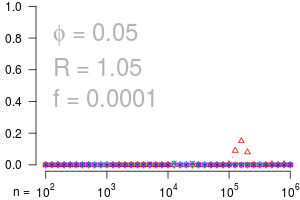
\includegraphics[width=0.26\textwidth]{simulation_plots/compare_tests/phi=005_R=105_f=1e-04.png}
        }%
        \subfigure{%
            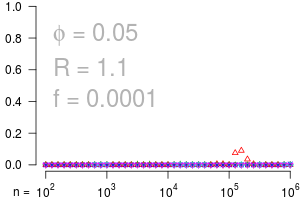
\includegraphics[width=0.26\textwidth]{simulation_plots/compare_tests/phi=005_R=110_f=1e-04.png}
        }%
        \subfigure{%
            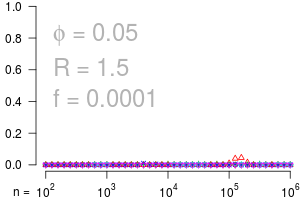
\includegraphics[width=0.26\textwidth]{simulation_plots/compare_tests/phi=005_R=150_f=1e-04.png}
        }\\ %  ------- End of the first row ----------------------%
        \subfigure{%
           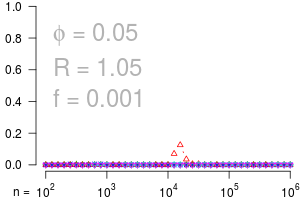
\includegraphics[width=0.26\textwidth]{simulation_plots/compare_tests/phi=005_R=105_f=0001.png}
        }%
        \subfigure{%
           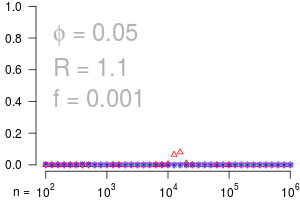
\includegraphics[width=0.26\textwidth]{simulation_plots/compare_tests/phi=005_R=110_f=0001.png}
        }%
        \subfigure{%
           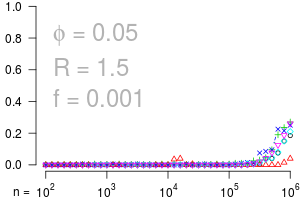
\includegraphics[width=0.26\textwidth]{simulation_plots/compare_tests/phi=005_R=150_f=0001.png}
        }\\ %  ------- End of the second row ----------------------%
        \subfigure{%
            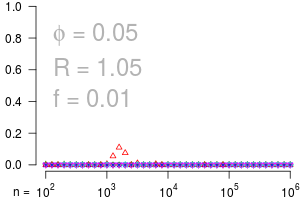
\includegraphics[width=0.26\textwidth]{simulation_plots/compare_tests/phi=005_R=105_f=001.png}
        }%
        \subfigure{%
            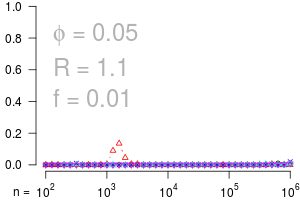
\includegraphics[width=0.26\textwidth]{simulation_plots/compare_tests/phi=005_R=110_f=001.png}
        }%
        \subfigure{%
            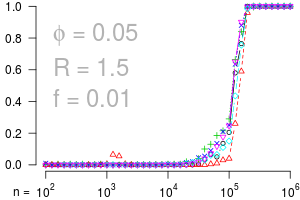
\includegraphics[width=0.26\textwidth]{simulation_plots/compare_tests/phi=005_R=150_f=001.png}
        }\\ %  ------- End of the third row ----------------------%
        \subfigure{%
            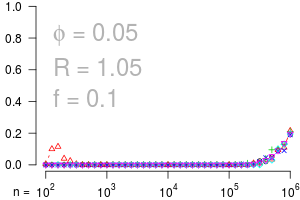
\includegraphics[width=0.26\textwidth]{simulation_plots/compare_tests/phi=005_R=105_f=01.png}
        }%
        \subfigure{%
            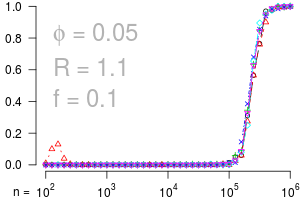
\includegraphics[width=0.26\textwidth]{simulation_plots/compare_tests/phi=005_R=110_f=01.png}
        }%
        \subfigure{%
            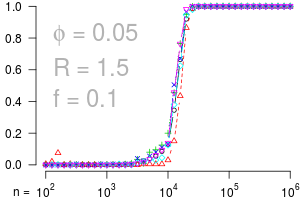
\includegraphics[width=0.26\textwidth]{simulation_plots/compare_tests/phi=005_R=150_f=01.png}
        }\\ %  ------- End of the fourth row ----------------------%
        \subfigure{%
            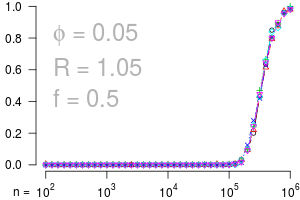
\includegraphics[width=0.26\textwidth]{simulation_plots/compare_tests/phi=005_R=105_f=05.png}
        }%
        \subfigure{%
            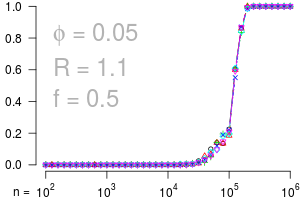
\includegraphics[width=0.26\textwidth]{simulation_plots/compare_tests/phi=005_R=110_f=05.png}
        }%
        \subfigure{%
            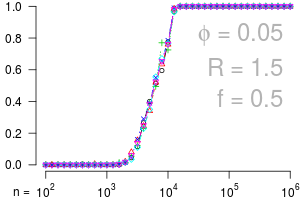
\includegraphics[width=0.26\textwidth]{simulation_plots/compare_tests/phi=005_R=150_f=05.png}
        }\\ %  ------- End of the fifth row ----------------------%
        \subfigure{%
            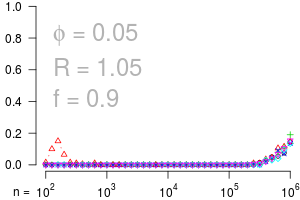
\includegraphics[width=0.26\textwidth]{simulation_plots/compare_tests/phi=005_R=105_f=09.png}
        }%
        \subfigure{%
            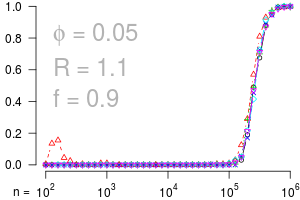
\includegraphics[width=0.26\textwidth]{simulation_plots/compare_tests/phi=005_R=110_f=09.png}
        }%
        \subfigure{%
            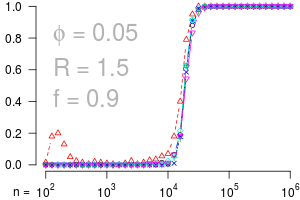
\includegraphics[width=0.26\textwidth]{simulation_plots/compare_tests/phi=005_R=150_f=09.png}
        }%
\caption{Empirical power as a function of sample sizes, under small to moderate odds ratios (left to right panels), and under rare to common risk allele frequencies (top to bottom panels).
The Fisher's exact test (black circles), Welch's t-test (red triangles), Pearson's chi-square test (blue crosses), Likelihood ratio test, and equivalently, LR test with logistic regression (light blue diamonds) are almost identical to the theoretical predictions (purple nabla), at sample sizes ranging from 100 to 100,000. Fraction of cases $\phi = 5\%$.
}\label{fig:compare-phi005}
\end{figure*}
\fi


\begin{figure*}[!tpb]
\centering
        \subfigure{%
            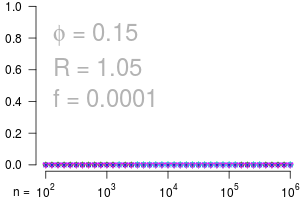
\includegraphics[width=0.26\textwidth]{simulation_plots/compare_tests/phi=015_R=105_f=1e-04.png}
        }%
        \subfigure{%
            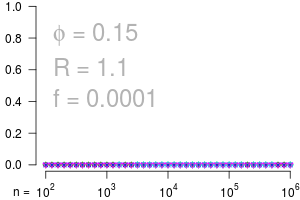
\includegraphics[width=0.26\textwidth]{simulation_plots/compare_tests/phi=015_R=110_f=1e-04.png}
        }%
        \subfigure{%
            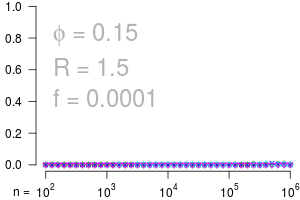
\includegraphics[width=0.26\textwidth]{simulation_plots/compare_tests/phi=015_R=150_f=1e-04.png}
        }\\ %  ------- End of the first row ----------------------%
        \subfigure{%
           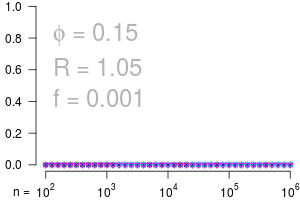
\includegraphics[width=0.26\textwidth]{simulation_plots/compare_tests/phi=015_R=105_f=0001.png}
        }%
        \subfigure{%
           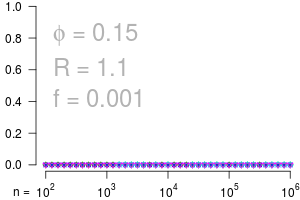
\includegraphics[width=0.26\textwidth]{simulation_plots/compare_tests/phi=015_R=110_f=0001.png}
        }%
        \subfigure{%
           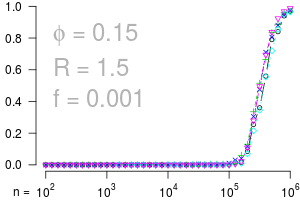
\includegraphics[width=0.26\textwidth]{simulation_plots/compare_tests/phi=015_R=150_f=0001.png}
        }\\ %  ------- End of the second row ----------------------%
        \subfigure{%
            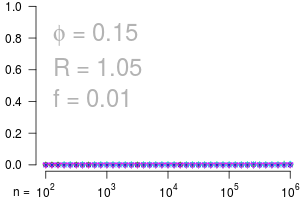
\includegraphics[width=0.26\textwidth]{simulation_plots/compare_tests/phi=015_R=105_f=001.png}
        }%
        \subfigure{%
            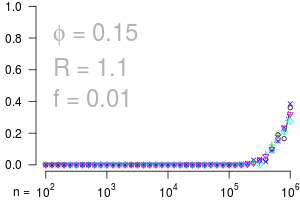
\includegraphics[width=0.26\textwidth]{simulation_plots/compare_tests/phi=015_R=110_f=001.png}
        }%
        \subfigure{%
            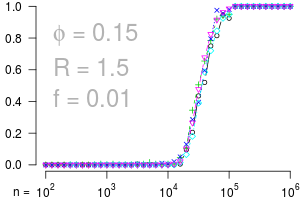
\includegraphics[width=0.26\textwidth]{simulation_plots/compare_tests/phi=015_R=150_f=001.png}
        }\\ %  ------- End of the third row ----------------------%
        \subfigure{%
            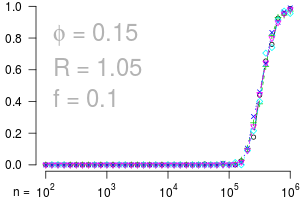
\includegraphics[width=0.26\textwidth]{simulation_plots/compare_tests/phi=015_R=105_f=01.png}
        }%
        \subfigure{%
            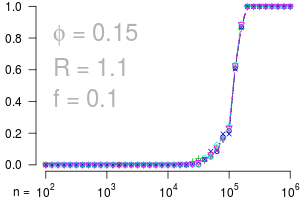
\includegraphics[width=0.26\textwidth]{simulation_plots/compare_tests/phi=015_R=110_f=01.png}
        }%
        \subfigure{%
            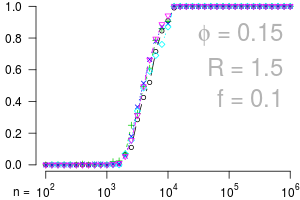
\includegraphics[width=0.26\textwidth]{simulation_plots/compare_tests/phi=015_R=150_f=01.png}
        }\\ %  ------- End of the fourth row ----------------------%
        \subfigure{%
            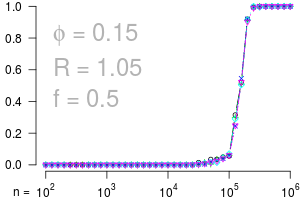
\includegraphics[width=0.26\textwidth]{simulation_plots/compare_tests/phi=015_R=105_f=05.png}
        }%
        \subfigure{%
            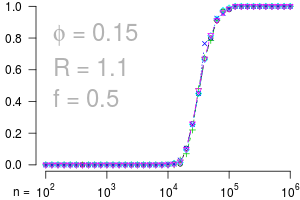
\includegraphics[width=0.26\textwidth]{simulation_plots/compare_tests/phi=015_R=110_f=05.png}
        }%
        \subfigure{%
            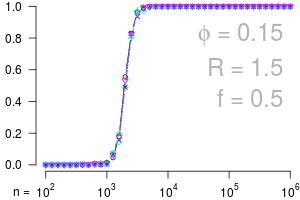
\includegraphics[width=0.26\textwidth]{simulation_plots/compare_tests/phi=015_R=150_f=05.png}
        }\\ %  ------- End of the fifth row ----------------------%
        \subfigure{%
            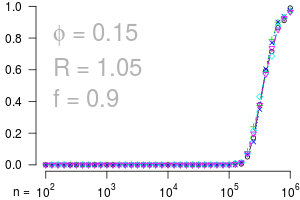
\includegraphics[width=0.26\textwidth]{simulation_plots/compare_tests/phi=015_R=105_f=09.png}
        }%
        \subfigure{%
            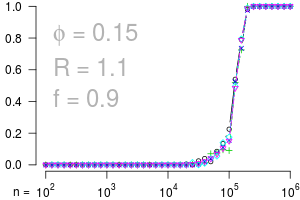
\includegraphics[width=0.26\textwidth]{simulation_plots/compare_tests/phi=015_R=110_f=09.png}
        }%
        \subfigure{%
            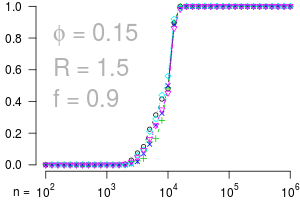
\includegraphics[width=0.26\textwidth]{simulation_plots/compare_tests/phi=015_R=150_f=09.png}
        }%
\caption{Empirical power as a function of sample sizes, under small to moderate odds ratios (left to right panels), and under rare to common risk allele frequencies (top to bottom panels).
The Fisher's exact test (black circles), Welch's t-test (red triangles), Pearson's chi-square test (blue crosses), Likelihood ratio test, and equivalently, LR test with logistic regression (light blue diamonds) are almost identical to the theoretical predictions (purple nabla), at sample sizes ranging from 100 to 100,000. Fraction of cases $\phi = 15\%$.
}\label{fig:compare-phi015}
\end{figure*}


\begin{figure*}[!tpb]
\centering
        \subfigure{%
            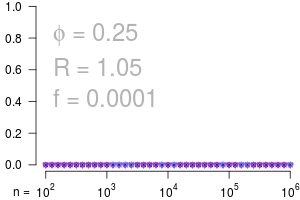
\includegraphics[width=0.26\textwidth]{simulation_plots/compare_tests/phi=025_R=105_f=1e-04.png}
        }%
        \subfigure{%
            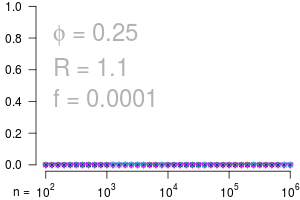
\includegraphics[width=0.26\textwidth]{simulation_plots/compare_tests/phi=025_R=110_f=1e-04.png}
        }%
        \subfigure{%
            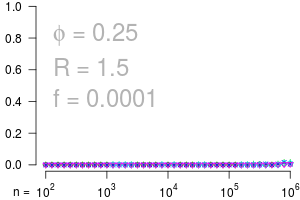
\includegraphics[width=0.26\textwidth]{simulation_plots/compare_tests/phi=025_R=150_f=1e-04.png}
        }\\ %  ------- End of the first row ----------------------%
        \subfigure{%
           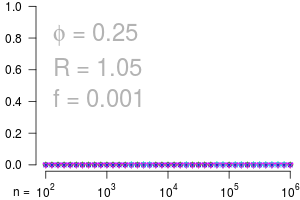
\includegraphics[width=0.26\textwidth]{simulation_plots/compare_tests/phi=025_R=105_f=0001.png}
        }%
        \subfigure{%
           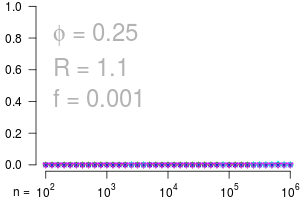
\includegraphics[width=0.26\textwidth]{simulation_plots/compare_tests/phi=025_R=110_f=0001.png}
        }%
        \subfigure{%
           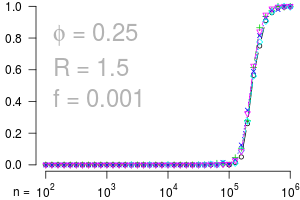
\includegraphics[width=0.26\textwidth]{simulation_plots/compare_tests/phi=025_R=150_f=0001.png}
        }\\ %  ------- End of the second row ----------------------%
        \subfigure{%
            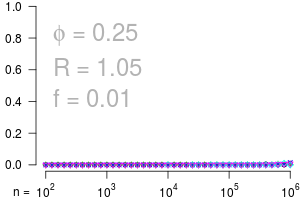
\includegraphics[width=0.26\textwidth]{simulation_plots/compare_tests/phi=025_R=105_f=001.png}
        }%
        \subfigure{%
            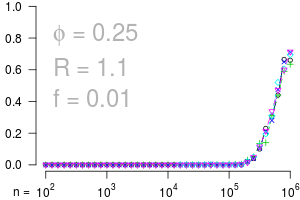
\includegraphics[width=0.26\textwidth]{simulation_plots/compare_tests/phi=025_R=110_f=001.png}
        }%
        \subfigure{%
            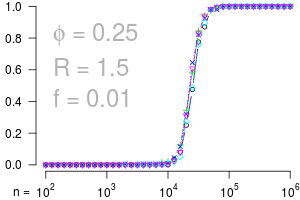
\includegraphics[width=0.26\textwidth]{simulation_plots/compare_tests/phi=025_R=150_f=001.png}
        }\\ %  ------- End of the third row ----------------------%
        \subfigure{%
            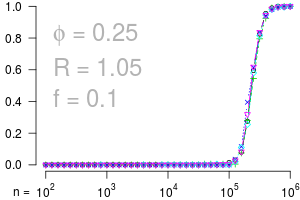
\includegraphics[width=0.26\textwidth]{simulation_plots/compare_tests/phi=025_R=105_f=01.png}
        }%
        \subfigure{%
            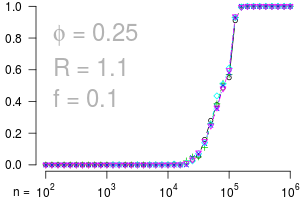
\includegraphics[width=0.26\textwidth]{simulation_plots/compare_tests/phi=025_R=110_f=01.png}
        }%
        \subfigure{%
            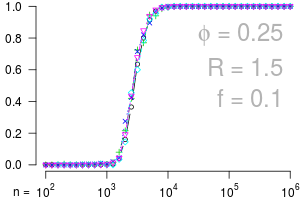
\includegraphics[width=0.26\textwidth]{simulation_plots/compare_tests/phi=025_R=150_f=01.png}
        }\\ %  ------- End of the fourth row ----------------------%
        \subfigure{%
            \includegraphics[width=0.26\textwidth]{simulation_plots/compare_tests/phi=025_R=105_f=05.png}
        }%
        \subfigure{%
            \includegraphics[width=0.26\textwidth]{simulation_plots/compare_tests/phi=025_R=110_f=05.png}
        }%
        \subfigure{%
            \includegraphics[width=0.26\textwidth]{simulation_plots/compare_tests/phi=025_R=150_f=05.png}
        }\\ %  ------- End of the fifth row ----------------------%
        \subfigure{%
            \includegraphics[width=0.26\textwidth]{simulation_plots/compare_tests/phi=025_R=105_f=09.png}
        }%
        \subfigure{%
            \includegraphics[width=0.26\textwidth]{simulation_plots/compare_tests/phi=025_R=110_f=09.png}
        }%
        \subfigure{%
            \includegraphics[width=0.26\textwidth]{simulation_plots/compare_tests/phi=025_R=150_f=09.png}
        }%
\caption{Empirical power as a function of sample sizes, under small to moderate odds ratios (left to right panels), and under rare to common risk allele frequencies (top to bottom panels).
The Fisher's exact test (black circles), Welch's t-test (red triangles), Pearson's chi-square test (blue crosses), Likelihood ratio test, and equivalently, LR test with logistic regression (light blue diamonds) are almost identical to the theoretical predictions (purple nabla), at sample sizes ranging from 100 to 100,000. Fraction of cases $\phi = 25\%$.
}\label{fig:compare-phi025}
\end{figure*}


\begin{figure*}[!tpb]
\centering
        \subfigure{%
            \includegraphics[width=0.26\textwidth]{simulation_plots/compare_tests/phi=035_R=105_f=1e-04.png}
        }%
        \subfigure{%
            \includegraphics[width=0.26\textwidth]{simulation_plots/compare_tests/phi=035_R=110_f=1e-04.png}
        }%
        \subfigure{%
            \includegraphics[width=0.26\textwidth]{simulation_plots/compare_tests/phi=035_R=150_f=1e-04.png}
        }\\ %  ------- End of the first row ----------------------%
        \subfigure{%
           \includegraphics[width=0.26\textwidth]{simulation_plots/compare_tests/phi=035_R=105_f=0001.png}
        }%
        \subfigure{%
           \includegraphics[width=0.26\textwidth]{simulation_plots/compare_tests/phi=035_R=110_f=0001.png}
        }%
        \subfigure{%
           \includegraphics[width=0.26\textwidth]{simulation_plots/compare_tests/phi=035_R=150_f=0001.png}
        }\\ %  ------- End of the second row ----------------------%
        \subfigure{%
            \includegraphics[width=0.26\textwidth]{simulation_plots/compare_tests/phi=035_R=105_f=001.png}
        }%
        \subfigure{%
            \includegraphics[width=0.26\textwidth]{simulation_plots/compare_tests/phi=035_R=110_f=001.png}
        }%
        \subfigure{%
            \includegraphics[width=0.26\textwidth]{simulation_plots/compare_tests/phi=035_R=150_f=001.png}
        }\\ %  ------- End of the third row ----------------------%
        \subfigure{%
            \includegraphics[width=0.26\textwidth]{simulation_plots/compare_tests/phi=035_R=105_f=01.png}
        }%
        \subfigure{%
            \includegraphics[width=0.26\textwidth]{simulation_plots/compare_tests/phi=035_R=110_f=01.png}
        }%
        \subfigure{%
            \includegraphics[width=0.26\textwidth]{simulation_plots/compare_tests/phi=035_R=150_f=01.png}
        }\\ %  ------- End of the fourth row ----------------------%
        \subfigure{%
            \includegraphics[width=0.26\textwidth]{simulation_plots/compare_tests/phi=035_R=105_f=05.png}
        }%
        \subfigure{%
            \includegraphics[width=0.26\textwidth]{simulation_plots/compare_tests/phi=035_R=110_f=05.png}
        }%
        \subfigure{%
            \includegraphics[width=0.26\textwidth]{simulation_plots/compare_tests/phi=035_R=150_f=05.png}
        }\\ %  ------- End of the fifth row ----------------------%
        \subfigure{%
            \includegraphics[width=0.26\textwidth]{simulation_plots/compare_tests/phi=035_R=105_f=09.png}
        }%
        \subfigure{%
            \includegraphics[width=0.26\textwidth]{simulation_plots/compare_tests/phi=035_R=110_f=09.png}
        }%
        \subfigure{%
            \includegraphics[width=0.26\textwidth]{simulation_plots/compare_tests/phi=035_R=150_f=09.png}
        }%
\caption{Empirical power as a function of sample sizes, under small to moderate odds ratios (left to right panels), and under rare to common risk allele frequencies (top to bottom panels).
The Fisher's exact test (black circles), Welch's t-test (red triangles), Pearson's chi-square test (blue crosses), Likelihood ratio test, and equivalently, LR test with logistic regression (light blue diamonds) are almost identical to the theoretical predictions (purple nabla), at sample sizes ranging from 100 to 100,000. Fraction of cases $\phi = 35\%$.
}\label{fig:compare-phi035}
\end{figure*}


\begin{figure*}[!tpb]
\centering
        \subfigure{%
            \includegraphics[width=0.26\textwidth]{simulation_plots/compare_tests/phi=050_R=105_f=1e-04.png}
        }%
        \subfigure{%
            \includegraphics[width=0.26\textwidth]{simulation_plots/compare_tests/phi=050_R=110_f=1e-04.png}
        }%
        \subfigure{%
            \includegraphics[width=0.26\textwidth]{simulation_plots/compare_tests/phi=050_R=150_f=1e-04.png}
        }\\ %  ------- End of the first row ----------------------%
        \subfigure{%
           \includegraphics[width=0.26\textwidth]{simulation_plots/compare_tests/phi=050_R=105_f=0001.png}
        }%
        \subfigure{%
           \includegraphics[width=0.26\textwidth]{simulation_plots/compare_tests/phi=050_R=110_f=0001.png}
        }%
        \subfigure{%
           \includegraphics[width=0.26\textwidth]{simulation_plots/compare_tests/phi=050_R=150_f=0001.png}
        }\\ %  ------- End of the second row ----------------------%
        \subfigure{%
            \includegraphics[width=0.26\textwidth]{simulation_plots/compare_tests/phi=050_R=105_f=001.png}
        }%
        \subfigure{%
            \includegraphics[width=0.26\textwidth]{simulation_plots/compare_tests/phi=050_R=110_f=001.png}
        }%
        \subfigure{%
            \includegraphics[width=0.26\textwidth]{simulation_plots/compare_tests/phi=050_R=150_f=001.png}
        }\\ %  ------- End of the third row ----------------------%
        \subfigure{%
            \includegraphics[width=0.26\textwidth]{simulation_plots/compare_tests/phi=050_R=105_f=01.png}
        }%
        \subfigure{%
            \includegraphics[width=0.26\textwidth]{simulation_plots/compare_tests/phi=050_R=110_f=01.png}
        }%
        \subfigure{%
            \includegraphics[width=0.26\textwidth]{simulation_plots/compare_tests/phi=050_R=150_f=01.png}
        }\\ %  ------- End of the fourth row ----------------------%
        \subfigure{%
            \includegraphics[width=0.26\textwidth]{simulation_plots/compare_tests/phi=050_R=105_f=05.png}
        }%
        \subfigure{%
            \includegraphics[width=0.26\textwidth]{simulation_plots/compare_tests/phi=050_R=110_f=05.png}
        }%
        \subfigure{%
            \includegraphics[width=0.26\textwidth]{simulation_plots/compare_tests/phi=050_R=150_f=05.png}
        }\\ %  ------- End of the fifth row ----------------------%
        \subfigure{%
            \includegraphics[width=0.26\textwidth]{simulation_plots/compare_tests/phi=050_R=105_f=09.png}
        }%
        \subfigure{%
            \includegraphics[width=0.26\textwidth]{simulation_plots/compare_tests/phi=050_R=110_f=09.png}
        }%
        \subfigure{%
            \includegraphics[width=0.26\textwidth]{simulation_plots/compare_tests/phi=050_R=150_f=09.png}
        }%
\caption{Empirical power as a function of sample sizes, under small to moderate odds ratios (left to right panels), and under rare to common risk allele frequencies (top to bottom panels).
The Fisher's exact test (black circles), Welch's t-test (red triangles), Pearson's chi-square test (blue crosses), Likelihood ratio test, and equivalently, LR test with logistic regression (light blue diamonds) are almost identical to the theoretical predictions (purple nabla), at sample sizes ranging from 100 to 100,000. Fraction of cases $\phi = 50\%$.
}\label{fig:compare-phi050}
\end{figure*}


\begin{figure*}[!tpb]
\centering
        \subfigure{%
            \includegraphics[width=0.26\textwidth]{simulation_plots/compare_tests/phi=085_R=105_f=1e-04.png}
        }%
        \subfigure{%
            \includegraphics[width=0.26\textwidth]{simulation_plots/compare_tests/phi=085_R=110_f=1e-04.png}
        }%
        \subfigure{%
            \includegraphics[width=0.26\textwidth]{simulation_plots/compare_tests/phi=085_R=150_f=1e-04.png}
        }\\ %  ------- End of the first row ----------------------%
        \subfigure{%
           \includegraphics[width=0.26\textwidth]{simulation_plots/compare_tests/phi=085_R=105_f=0001.png}
        }%
        \subfigure{%
           \includegraphics[width=0.26\textwidth]{simulation_plots/compare_tests/phi=085_R=110_f=0001.png}
        }%
        \subfigure{%
           \includegraphics[width=0.26\textwidth]{simulation_plots/compare_tests/phi=085_R=150_f=0001.png}
        }\\ %  ------- End of the second row ----------------------%
        \subfigure{%
            \includegraphics[width=0.26\textwidth]{simulation_plots/compare_tests/phi=085_R=105_f=001.png}
        }%
        \subfigure{%
            \includegraphics[width=0.26\textwidth]{simulation_plots/compare_tests/phi=085_R=110_f=001.png}
        }%
        \subfigure{%
            \includegraphics[width=0.26\textwidth]{simulation_plots/compare_tests/phi=085_R=150_f=001.png}
        }\\ %  ------- End of the third row ----------------------%
        \subfigure{%
            \includegraphics[width=0.26\textwidth]{simulation_plots/compare_tests/phi=085_R=105_f=01.png}
        }%
        \subfigure{%
            \includegraphics[width=0.26\textwidth]{simulation_plots/compare_tests/phi=085_R=110_f=01.png}
        }%
        \subfigure{%
            \includegraphics[width=0.26\textwidth]{simulation_plots/compare_tests/phi=085_R=150_f=01.png}
        }\\ %  ------- End of the fourth row ----------------------%
        \subfigure{%
            \includegraphics[width=0.26\textwidth]{simulation_plots/compare_tests/phi=085_R=105_f=05.png}
        }%
        \subfigure{%
            \includegraphics[width=0.26\textwidth]{simulation_plots/compare_tests/phi=085_R=110_f=05.png}
        }%
        \subfigure{%
            \includegraphics[width=0.26\textwidth]{simulation_plots/compare_tests/phi=085_R=150_f=05.png}
        }\\ %  ------- End of the fifth row ----------------------%
        \subfigure{%
            \includegraphics[width=0.26\textwidth]{simulation_plots/compare_tests/phi=085_R=105_f=09.png}
        }%
        \subfigure{%
            \includegraphics[width=0.26\textwidth]{simulation_plots/compare_tests/phi=085_R=110_f=09.png}
        }%
        \subfigure{%
            \includegraphics[width=0.26\textwidth]{simulation_plots/compare_tests/phi=085_R=150_f=09.png}
        }%
\caption{Empirical power as a function of sample sizes, under small to moderate odds ratios (left to right panels), and under rare to common risk allele frequencies (top to bottom panels).
The Fisher's exact test (black circles), Welch's t-test (red triangles), Pearson's chi-square test (blue crosses), Likelihood ratio test, and equivalently, LR test with logistic regression (light blue diamonds) are almost identical to the theoretical predictions (purple nabla), at sample sizes ranging from 100 to 100,000. Fraction of cases $\phi = 85\%$.
}\label{fig:compare-phi085}
\end{figure*}

\subsection{Power as a function of the canonical parameters}

To fully explore the accuracy of the theoretical predictions, we extend the simulation to a wider range of model parameters.
\begin{itemize}
    \item Sample size total, $n$: $10^2$, $10^3$, $10^4$, $10^5$,
    \item Fraction of cases in the study, $\phi$: $5\%$, $15\%$, $25\%$ $50\%$, $85\%$,
    \item Risk allele frequencies in control group, $f$: a grid of $100$ values ranging from $0.01\%$ to $99.5\%$. The values are non-regularly spaced; more values are selected towards the end points of the interval $(0,1)$.
    \item Odds ratio, $R$: a grid of $100$ values ranging from $1$ to $100$. The values are regularly spaced on the log-scale.
    \item p-value cutoffs: $5\times 10^{-5}$, $5\times 10^{-8}$.
\end{itemize}
Each of the $4\times4\times100\times100\times2$ parameter value combinations were simulated $1000$ times.

We compare the theoretical results with powers of Fisher's exact test obtained by simulations.
We choose to compare against exact tests for their superior performance in finite samples ---
while approximate tests like the chi-square test and likelihood ratio tests may fail to protect against type I error inflation when sample sizes are small, exact tests maintain the correct levels. 

The results for p-value cutoff at $5\times 10^{-8}$ are visualized in the form ``OR-RAF diagrams'' to better highlight settings under which the theoretical predictions and the empirical powers differ.

\begin{figure*}[!tpb]%figure1
\centering
        \subfigure{%
            \includegraphics[width=0.30\textwidth]{simulation_plots/phase_diagram/n100_phi005_p5e-8_theoretical.png}
        }%
        \subfigure{%
           \includegraphics[width=0.30\textwidth]{simulation_plots/phase_diagram/n100_phi005_p5e-8.png}
        }%
        \subfigure{%
            \includegraphics[width=0.30\textwidth]{simulation_plots/phase_diagram/n100_phi005_p5e-8_diff.png}
        } \\ %  ------- End of the first row ----------------------%
        \subfigure{%
            \includegraphics[width=0.30\textwidth]{simulation_plots/phase_diagram/n1000_phi005_p5e-8_theoretical.png}
        }%
        \subfigure{%
            \includegraphics[width=0.30\textwidth]{simulation_plots/phase_diagram/n1000_phi005_p5e-8.png}
        }%
        \subfigure{%
            \includegraphics[width=0.30\textwidth]{simulation_plots/phase_diagram/n1000_phi005_p5e-8_diff.png}
        } \\ %  ------- End of the second row ----------------------%
        \subfigure{%
            \includegraphics[width=0.30\textwidth]{simulation_plots/phase_diagram/n10000_phi005_p5e-8_theoretical.png}
        }%
        \subfigure{%
            \includegraphics[width=0.30\textwidth]{simulation_plots/phase_diagram/n10000_phi005_p5e-8.png}
        }%
        \subfigure{%
            \includegraphics[width=0.30\textwidth]{simulation_plots/phase_diagram/n10000_phi005_p5e-8_diff.png}
        } \\ %  ------- End of the third row ----------------------%
        \subfigure{%
            \includegraphics[width=0.30\textwidth]{simulation_plots/phase_diagram/n100000_phi005_p5e-8_theoretical.png}
        }%
        \subfigure{%
            \includegraphics[width=0.30\textwidth]{simulation_plots/phase_diagram/n100000_phi005_p5e-8.png}
        }%
        \subfigure{%
            \includegraphics[width=0.30\textwidth]{simulation_plots/phase_diagram/n100000_phi005_p5e-8_diff.png}
        }
\caption{
Statistical powers for the OR-RAF combinations, obtained from theoretical predictions (left column) and by simulations (middle column). Their absolute differences (right column) are shown at sample sizes ranging from $100$ to $100,000$ (top to bottom).
p-value threshold is at $5\times10^{-8}$.
Fractions of cases $\phi=5\%$.
}\label{fig:phi005}
\end{figure*}

\begin{figure*}[!tpb]%figure1
\centering
        \subfigure{%
            \includegraphics[width=0.30\textwidth]{simulation_plots/phase_diagram/n100_phi015_p5e-8_theoretical.png}
        }%
        \subfigure{%
           \includegraphics[width=0.30\textwidth]{simulation_plots/phase_diagram/n100_phi015_p5e-8.png}
        }%
        \subfigure{%
            \includegraphics[width=0.30\textwidth]{simulation_plots/phase_diagram/n100_phi015_p5e-8_diff.png}
        } \\ %  ------- End of the first row ----------------------%
        \subfigure{%
            \includegraphics[width=0.30\textwidth]{simulation_plots/phase_diagram/n1000_phi015_p5e-8_theoretical.png}
        }%
        \subfigure{%
            \includegraphics[width=0.30\textwidth]{simulation_plots/phase_diagram/n1000_phi015_p5e-8.png}
        }%
        \subfigure{%
            \includegraphics[width=0.30\textwidth]{simulation_plots/phase_diagram/n1000_phi015_p5e-8_diff.png}
        } \\ %  ------- End of the second row ----------------------%
        \subfigure{%
            \includegraphics[width=0.30\textwidth]{simulation_plots/phase_diagram/n10000_phi015_p5e-8_theoretical.png}
        }%
        \subfigure{%
            \includegraphics[width=0.30\textwidth]{simulation_plots/phase_diagram/n10000_phi015_p5e-8.png}
        }%
        \subfigure{%
            \includegraphics[width=0.30\textwidth]{simulation_plots/phase_diagram/n10000_phi015_p5e-8_diff.png}
        } \\ %  ------- End of the third row ----------------------%
        \subfigure{%
            \includegraphics[width=0.30\textwidth]{simulation_plots/phase_diagram/n100000_phi015_p5e-8_theoretical.png}
        } %
        \subfigure{%
            \includegraphics[width=0.30\textwidth]{simulation_plots/phase_diagram/n100000_phi015_p5e-8.png}
        }%
        \subfigure{%
            \includegraphics[width=0.30\textwidth]{simulation_plots/phase_diagram/n100000_phi015_p5e-8_diff.png}
        } %
\caption{
Statistical powers for the OR-RAF combinations, obtained from theoretical predictions (left column) and by simulations (middle column). Their absolute differences (right column) are shown at sample sizes ranging from $100$ to $100,000$ (top to bottom).
p-value threshold is at $5\times10^{-8}$.
Fractions of cases $\phi=15\%$.
}\label{fig:phi015}
\end{figure*}

\begin{figure*}[!tpb]%figure1
\centering
        \subfigure{%
            \includegraphics[width=0.30\textwidth]{simulation_plots/phase_diagram/n100_phi025_p5e-8_theoretical.png}
        }%
        \subfigure{%
           \includegraphics[width=0.30\textwidth]{simulation_plots/phase_diagram/n100_phi025_p5e-8.png}
        }%
        \subfigure{%
            \includegraphics[width=0.30\textwidth]{simulation_plots/phase_diagram/n100_phi025_p5e-8_diff.png}
        } \\ %  ------- End of the first row ----------------------%
        \subfigure{%
            \includegraphics[width=0.30\textwidth]{simulation_plots/phase_diagram/n1000_phi025_p5e-8_theoretical.png}
        }%
        \subfigure{%
            \includegraphics[width=0.30\textwidth]{simulation_plots/phase_diagram/n1000_phi025_p5e-8.png}
        }%
        \subfigure{%
            \includegraphics[width=0.30\textwidth]{simulation_plots/phase_diagram/n1000_phi025_p5e-8_diff.png}
        } \\ %  ------- End of the second row ----------------------%
        \subfigure{%
            \includegraphics[width=0.30\textwidth]{simulation_plots/phase_diagram/n10000_phi025_p5e-8_theoretical.png}
        }%
        \subfigure{%
            \includegraphics[width=0.30\textwidth]{simulation_plots/phase_diagram/n10000_phi025_p5e-8.png}
        }%
        \subfigure{%
            \includegraphics[width=0.30\textwidth]{simulation_plots/phase_diagram/n10000_phi025_p5e-8_diff.png}
        } \\ %  ------- End of the third row ----------------------%
        \subfigure{%
            \includegraphics[width=0.30\textwidth]{simulation_plots/phase_diagram/n100000_phi025_p5e-8_theoretical.png}
        }%
        \subfigure{%
            \includegraphics[width=0.30\textwidth]{simulation_plots/phase_diagram/n100000_phi025_p5e-8.png}
        }%
        \subfigure{%
            \includegraphics[width=0.30\textwidth]{simulation_plots/phase_diagram/n100000_phi025_p5e-8_diff.png}
        } %
\caption{
Statistical powers for the OR-RAF combinations, obtained from theoretical predictions (left column) and by simulations (middle column). Their absolute differences (right column) are shown at sample sizes ranging from $100$ to $100,000$ (top to bottom).
p-value threshold is at $5\times10^{-8}$.
Fractions of cases $\phi=25\%$.
}\label{fig:phi025}
\end{figure*}


\begin{figure*}[!tpb]%figure1
\centering
        \subfigure{%
            \includegraphics[width=0.30\textwidth]{simulation_plots/phase_diagram/n100_phi05_p5e-8_theoretical.png}
        }%
        \subfigure{%
           \includegraphics[width=0.30\textwidth]{simulation_plots/phase_diagram/n100_phi05_p5e-8.png}
        }%
        \subfigure{%
            \includegraphics[width=0.30\textwidth]{simulation_plots/phase_diagram/n100_phi05_p5e-8_diff.png}
        } \\ %  ------- End of the first row ----------------------%
        \subfigure{%
            \includegraphics[width=0.30\textwidth]{simulation_plots/phase_diagram/n1000_phi05_p5e-8_theoretical.png}
        }%
        \subfigure{%
            \includegraphics[width=0.30\textwidth]{simulation_plots/phase_diagram/n1000_phi05_p5e-8.png}
        }%
        \subfigure{%
            \includegraphics[width=0.30\textwidth]{simulation_plots/phase_diagram/n1000_phi05_p5e-8_diff.png}
        } \\ %  ------- End of the second row ----------------------%
        \subfigure{%
            \includegraphics[width=0.30\textwidth]{simulation_plots/phase_diagram/n10000_phi05_p5e-8_theoretical.png}
        }%
        \subfigure{%
            \includegraphics[width=0.30\textwidth]{simulation_plots/phase_diagram/n10000_phi05_p5e-8.png}
        }%
        \subfigure{%
            \includegraphics[width=0.30\textwidth]{simulation_plots/phase_diagram/n10000_phi05_p5e-8_diff.png}
        } \\ %  ------- End of the third row ----------------------%
        \subfigure{%
            \includegraphics[width=0.30\textwidth]{simulation_plots/phase_diagram/n100000_phi05_p5e-8_theoretical.png}
        }%
        \subfigure{%
            \includegraphics[width=0.30\textwidth]{simulation_plots/phase_diagram/n100000_phi05_p5e-8.png}
        }%
        \subfigure{%
            \includegraphics[width=0.30\textwidth]{simulation_plots/phase_diagram/n100000_phi05_p5e-8_diff.png}
        }
\caption{
Statistical powers for the OR-RAF combinations, obtained from theoretical predictions (left column) and by simulations (middle column). Their absolute differences (right column) are shown at sample sizes ranging from $100$ to $100,000$ (top to bottom).
p-value threshold is at $5\times10^{-8}$.
Fractions of cases $\phi=50\%$.
}\label{fig:phi05}
\end{figure*}

\begin{figure*}[!tpb]%figure1
\centering
        \subfigure{%
            \includegraphics[width=0.30\textwidth]{simulation_plots/phase_diagram/n100_phi085_p5e-8_theoretical.png}
        }%
        \subfigure{%
           \includegraphics[width=0.30\textwidth]{simulation_plots/phase_diagram/n100_phi085_p5e-8.png}
        }%
        \subfigure{%
            \includegraphics[width=0.30\textwidth]{simulation_plots/phase_diagram/n100_phi085_p5e-8_diff.png}
        } \\ %  ------- End of the first row ----------------------%
        \subfigure{%
            \includegraphics[width=0.30\textwidth]{simulation_plots/phase_diagram/n1000_phi085_p5e-8_theoretical.png}
        }%
        \subfigure{%
            \includegraphics[width=0.30\textwidth]{simulation_plots/phase_diagram/n1000_phi085_p5e-8.png}
        }%
        \subfigure{%
            \includegraphics[width=0.30\textwidth]{simulation_plots/phase_diagram/n1000_phi085_p5e-8_diff.png}
        } \\ %  ------- End of the second row ----------------------%
        \subfigure{%
            \includegraphics[width=0.30\textwidth]{simulation_plots/phase_diagram/n10000_phi085_p5e-8_theoretical.png}
        }%
        \subfigure{%
            \includegraphics[width=0.30\textwidth]{simulation_plots/phase_diagram/n10000_phi085_p5e-8.png}
        }%
        \subfigure{%
            \includegraphics[width=0.30\textwidth]{simulation_plots/phase_diagram/n10000_phi085_p5e-8_diff.png}
        } \\ %  ------- End of the third row ----------------------%
        \subfigure{%
            \includegraphics[width=0.30\textwidth]{simulation_plots/phase_diagram/n100000_phi085_p5e-8_theoretical.png}
        }%
        \subfigure{%
            \includegraphics[width=0.30\textwidth]{simulation_plots/phase_diagram/n100000_phi085_p5e-8.png}
        }%
        \subfigure{%
            \includegraphics[width=0.30\textwidth]{simulation_plots/phase_diagram/n100000_phi085_p5e-8_diff.png}
        } %
\caption{
Statistical powers for the OR-RAF combinations, obtained from theoretical predictions (left column) and by simulations (middle column). Their absolute differences (right column) are shown at sample sizes ranging from $100$ to $100,000$ (top to bottom).
p-value threshold is at $5\times10^{-8}$.
Fractions of cases $\phi=85\%$.
}\label{fig:phi085}
\end{figure*}


The results are shown in Figures \ref{fig:phi005} to \ref{fig:phi085}, organized by increasing fraction of cases in the study $\phi$.
Left columns of the figures show the theoretical predictions obtained by Theorem \ref{thm:1}, the middle columns shows the estimated powers from simulation, and the right columns visualize their differences.
Sample sizes ranging from $100$ to $100,000$ are arranged from top to bottom in each figure.


\subsection{Accuracy of theoretical predictions}
\label{subsec:accuracy-of-asymptotics}

% We now comment on some major features of the theoretical predictions.

We find that the asymptotic approximations in Theorem \ref{thm:1} to be robust for small to moderate odds ratios ($R<2$), as seen in all simulation studies (see Figures \ref{fig:compare-phi015} to \ref{fig:phi085}).

The theoretical approximations are extremely accurate (within 1 percentage point in absolute deviations) for balanced designs, even at very small sample sizes (see Figure \ref{fig:phi05}), as well as in settings with moderately more controls than controls at large sample sizes (see Figures \ref{fig:phi015} and \ref{fig:phi025}, $n=100,000$).
Some discrepancies can be seen under designs with too few cases (see Figure \ref{fig:phi005}) as well as too few controls (see Figure \ref{fig:phi085}), although the differences vanish as the sample sizes increase.

\begin{table}[h]
\begin{center}
    \begin{tabular}{cccccc}
    \hline
        & \multicolumn{5}{c}{Fraction of cases $\phi$} \\
        \cline{2-6}
        sample size $n$ & $5\%$ & $15\%$ & $25\%$ & $50\%$ & $85\%$ \\
        \hline
        $100$ & 4.61 (0.15) & 2.39 (0.08) & 1.44 (0.05) & 0.78 (0.02) & 2.00 (0.07) \\
        $1,000$ & 5.01 (0.15) & 3.37 (0.10) & 2.35 (0.7) & 1.03 (0.03) & 3.44 (0.10) \\
        $10,000$ & 4.73 (0.14) & 3.06 (0.09) & 1.98 (0.07) & 0.50 (0.02) & 2.43 (0.08) \\
        $100,000$ & 1.74 (0.07) & 0.73 (0.03) & 0.43 (0.02) & 0.18 (0.01) & 0.88 (0.04) \\
    \hline
    \end{tabular}
    \caption{Mean absolute deviations in percentage points between the theoretical predictions and the simulated results, with standard errors in brackets. The p-values threshold are set at $5\times10^{-8}$.}
    \label{tbl:accuracy-of-asymptotic-power}
\end{center}
\end{table}


In general, the mismatch between the theoretical predictions and empirical power only takes place at small sample sizes, and only for large odds ratios ($R>3$).
% The proposed correction based on minimum calibration numbers seems to provide a simple resolution for this mismatch.
% Alternatives with expected allele counts less than required by the minimum calibration numbers (outside the red dashed lines) should be interpreted to have near zero power.
% That is, in the OR-RAF diagrams, regions outside the red dashed lines should also be colored dark.
% The corrected predictions are closer to what is obtained for exact tests.
For small odds ratios, numerical experiments suggest that our power calculations are robust across a wide range of case-control ratios and sample sizes.

Theoretical predictions for p-value cutoff at $5\times 10^{-5}$ are up to $20\%$ more accurate than for p-value cutoff at $5\times 10^{-8}$, but qualitatively similar.
For example, the average absolute deviation for unbalanced designs ($\phi=15\%$) at sample size $n=100,000$ is only $0.57$ percentage points for p-value cutoff at $5\times 10^{-5}$, down from $0.73$ percentage points when p-value cutoff is at $5\times 10^{-8}$.
The same metric improves to $0.16$, down from $0.18$ percentage points, for balanced designs ($\phi=50\%$) at the same sample sizes.
In the interest of space, we only show the more challenging cases where the p-value cutoffs are set at $5\times 10^{-8}$.

For sample sizes beyond $100,000$ (not reported), we find the empirical power to be almost indistinguishable from theoretical predictions.



% \section{An errata for Johnson et~al.\ (2017)}
% \label{sec:errata}
% We identify an error in the software implementation of \citet{Johnson17}.

In particular, \citet{Johnson17} specify the alternative hypothesis with a disease model (additive, dominant, etc.), disease prevalence $K$, and the risk allele frequency \emph{in the population} $q$ (notice that this differs from our definition, and from the reporting standard of NHGRI-EBI GWAS Catalog). 

Assuming Hardy-Weinberg equilibrium, the expected frequency of genotypes $(aa, aA, AA)$ is $((1-q)^2, q(1-q), q^2)$.
The relative risks $R_{aA}$, $R_{AA}$ for the latter two genotypes are calculated based on the assumed disease model and the assumed relative risks $R_{aA}$.

By an application of Bayes' rule, the conditional probabilities of Cases, given the genotypes are
\begin{align}
    \mathbb P[\mathrm{Case}|aa] &= \frac{K}{(1-q)^2 + 2(1-q)qR_{aA} + q^2R_{AA}} \\
    \mathbb P[\mathrm{Case}|aA] &= \mathbb P[\mathrm{Case}|aa] \times R_{aA} \\
    \mathbb P[\mathrm{Case}|AA] &= \mathbb P[\mathrm{Case}|aa] \times R_{AA}.
\end{align}
A valid disease model dictates that each of these probabilities are between 0 and 1.


% \vspace*{-10pt}
% \section*{Acknowledgements}
% 
% We thank so and so for their invaluable comments and suggestions on the early versions of the software and this paper.

%\vspace{*{-12pt}
\section*{Funding}

This work is partially supported by NSF Grant DMS-1830293, Algorithms for Threat Detection.


%\bibliographystyle{natbib}
%\bibliographystyle{achemnat}
%\bibliographystyle{plainnat}
%\bibliographystyle{abbrv}
%\bibliographystyle{bioinformatics}
%
%\bibliographystyle{plain}
%
%\bibliography{Document}

%\vspace{*{-12pt}
\begin{thebibliography}{}

\normalsize{
\bibitem[Choi {\it et~al}., 2017]{Choi17}
Choi, L., Blume, J. D., \& Dupont, W. D. (2015). 
Elucidating the foundations of statistical inference with 2 x 2 tables. 
{\it PloS one}, {\bf 10(4)}, e0121263.

\bibitem[Derkach {\it et~al}., 2017]{Derkach17}
Derkach, A., Zhang, H., \& Chatterjee, N. (2017). 
Power Analysis for Genetic Association Test (PAGEANT) provides insights to challenges for rare variant association studies. 
{\it Bioinformatics}, {\bf 34(9)}, 1506-1513.

\bibitem[Dominguez-Cruz {\it et~al}., 2018]{Dominguez-Cruz18}
Dom\'inguez-Cruz, M. G., de Lourdes Mu\~noz, M., Totomoch-Serra, A., Garc\'ia-Escalante, M. G., Burgue\~no, J., Valadez-Gonz\'alez, N., ... \& D\'iaz-Badillo, \'A. (2018). 
Pilot genome-wide association study identifying novel risk loci for type 2 diabetes in a Maya population. 
{\it Gene}, {\bf 677}, 324-331.

\bibitem[Ferguson, 2017]{Ferguson17}
Ferguson, T. S. (2017). {\it A course in large sample theory}. Routledge.

\bibitem[Gonz\'{a}lez {\it et~al}., 2008]{Gonzalez08}
Gonz\'{a}lez, J. R., Carrasco, J. L., Dudbridge, F., Armengol, L., Estivill, X., \& Moreno, V. (2008). 
Maximizing association statistics over genetic models. 
{\it Genetic Epidemiology}, {\bf 32(3)}, 246-254.

\bibitem[Hunter, 2002]{Hunter02}
Hunter, D. (2002) Topic 25: Asymptotic Power of Pearson’s Chi-Square Test in 
{\it Statistics 597A: Asymptotic Tools (Fall 2002), PSU Lecture notes,} http://personal.psu.edu/drh20/asymp/fall2002/lectures/ln11.pdf

\bibitem[Johnson {\it et~al}., 2017]{Johnson17}
Johnson, J. L., \& Abecasis, G. R. (2017). 
GAS Power Calculator: web-based power calculator for genetic association studies. 
{\it bioRxiv}, 164343.

\bibitem[Lehmann, 2004]{Lehmann04}
Lehmann, E. L. (2004). {\it Elements of large-sample theory}. Springer Science \& Business Media.

\bibitem[Li {\it et~al}., 2008]{Li08}
Li, Q., Zheng, G., Li, Z., \& Yu, K. (2008). 
Efficient approximation of P‐value of the maximum of correlated tests, with applications to genome‐wide association studies. 
{\it Annals of human genetics}, {\bf 72(3)}, 397-406.

\bibitem[MacArthur {\it et~al}., 2016]{MacArthur16}
MacArthur, J., Bowler, E., Cerezo, M., Gil, L., Hall, P., Hastings, E., ... \& Pendlington, Z. M. (2016). 
The new NHGRI-EBI Catalog of published genome-wide association studies (GWAS Catalog). 
{\it Nucleic acids research}, {\bf 45(D1)}, D896-D901.

\bibitem[Menashe {\it et~al}., 2008]{Menashe08}
Menashe, I., Rosenberg, P. S., \& Chen, B. E. (2008). 
PGA: power calculator for case-control genetic association analyses. 
{\it BMC genetics}, {\bf 9(1)}, 36.

\bibitem[Purcell {\it et~al}., 2003]{Purcell03}
Purcell, S., Cherny, S. S., \& Sham, P. C. (2003). 
Genetic Power Calculator: design of linkage and association genetic mapping studies of complex traits. 
{\it Bioinformatics}, {\bf 19(1)}, 149-150.

\bibitem[Ripamonti {\it et~al}., 2017]{Ripamonti17}
Ripamonti, E., Lloyd, C., \& Quatto, P. (2017). 
Contemporary Frequentist Views of the $2\times2$ Binomial Trial. 
{\it Statistical Science}, {\bf 32(4)}, 600-615.

\bibitem[Sham, 1998]{Sham98}
Sham, P. C. (1998). {\it Statistics in human genetics}. Wiley.

\bibitem[Skol {\it et~al}., 2006]{Skol06}
Skol, A. D., Scott, L. J., Abecasis, G. R., \& Boehnke, M. (2006). 
Joint analysis is more efficient than replication-based analysis for two-stage genome-wide association studies. 
{\it Nature genetics}, {\bf 38(2)}, 209.

\bibitem[Smyth {\it et~al}., 2017]{Smyth17}
Smyth, G., Hu, Y., Dunn, P., Phipson, B., \& Chen, Y. (2017)
statmod: Statistical Modeling.
R package version 1.4.30.
%{\it https://cran.r-project.org/web/packages/statmod}.

\bibitem[Wang {\it et~al}., 2014]{Wang14}
Wang, G. T., Li, B., Lyn Santos-Cortez, R. P., Peng, B., \& Leal, S. M. (2014).
Power analysis and sample size estimation for sequence-based association studies. 
{\it Bioinformatics}, {\bf 30(16)}, 2377-2378.
}

\end{thebibliography}
\end{document}
